

\documentclass[11pt,fleqn]{book} % Default font size and left-justified equations

%%%%%%%%%%%%%%%%%%%%%%%%%%%%%%%%%%%%%%%%%
% The Legrand Orange Book
% Structural Definitions File
% Version 2.0 (9/2/15)
%
% Original author:
% Mathias Legrand (legrand.mathias@gmail.com) with modifications by:
% Vel (vel@latextemplates.com)
% 
% This file has been downloaded from:
% http://www.LaTeXTemplates.com
%
% License:
% CC BY-NC-SA 3.0 (http://creativecommons.org/licenses/by-nc-sa/3.0/)
%
%%%%%%%%%%%%%%%%%%%%%%%%%%%%%%%%%%%%%%%%%

%----------------------------------------------------------------------------------------
%	VARIOUS REQUIRED PACKAGES AND CONFIGURATIONS
%----------------------------------------------------------------------------------------

\usepackage[top=3cm,bottom=3cm,left=5.5cm,right=3cm,headsep=10pt,letterpaper,asymmetric]{geometry} % Page margins
% Could use 6cm margin on left 

\usepackage{graphicx} % Required for including pictures
\graphicspath{{Pictures/}} % Specifies the directory where pictures are stored

\usepackage{lipsum} % Inserts dummy text

\usepackage{tikz} % Required for drawing custom shapes

\usepackage[english]{babel} % English language/hyphenation

\usepackage{enumitem} % Customize lists
\setlist{noitemsep} % Reduce spacing between bullet points and numbered lists

\usepackage{booktabs} % Required for nicer horizontal rules in tables

\usepackage{xcolor} % Required for specifying colors by name
%\definecolor{rust}{RGB}{243,102,25} % Define the orange color used for highlighting throughout the book
\definecolor{rust}{RGB}{153, 0, 0} % Define alternate red color

\usepackage{pdftexcmds}



%----------------------------------------------------------------------------------------
%	FONTS
%----------------------------------------------------------------------------------------

\usepackage{avant} % Use the Avantgarde font for headings
%\usepackage{times} % Use the Times font for headings
\usepackage{mathptmx} % Use the Adobe Times Roman as the default text font together with math symbols from the Sym­bol, Chancery and Com­puter Modern fonts

\usepackage{microtype} % Slightly tweak font spacing for aesthetics
\usepackage[utf8]{inputenc} % Required for including letters with accents
\usepackage[T1]{fontenc} % Use 8-bit encoding that has 256 glyphs
\usepackage{relsize} % Allow relative font sizing
\renewcommand\RSlargest{100pt} 
%----------------------------------------------------------------------------------------
%	BIBLIOGRAPHY AND INDEX
%----------------------------------------------------------------------------------------

\usepackage[style=alphabetic,citestyle=numeric,sorting=nyt,sortcites=true,autopunct=true,babel=hyphen,hyperref=true,abbreviate=false,backref=true,backend=biber]{biblatex}
\addbibresource{bibliography.bib} % BibTeX bibliography file
\defbibheading{bibempty}{}

\usepackage{calc} % For simpler calculation - used for spacing the index letter headings correctly
\usepackage{makeidx} % Required to make an index
\makeindex % Tells LaTeX to create the files required for indexing

%----------------------------------------------------------------------------------------
%	MAIN TABLE OF CONTENTS
%----------------------------------------------------------------------------------------

\usepackage{titletoc} % Required for manipulating the table of contents

\contentsmargin{0cm} % Removes the default margin

% Part text styling
\titlecontents{part}[0cm]
{\addvspace{20pt}\centering\large\bfseries}
{}
{}
{}

% Chapter text styling
\titlecontents{chapter}[1.25cm] % Indentation
{\addvspace{12pt}\large\sffamily\bfseries} % Spacing and font options for chapters
{\color{rust!60}\contentslabel[\Large\thecontentslabel]{1.25cm}\color{rust}} % Chapter number
{\color{rust}}  
{\color{rust!60}\normalsize\;\titlerule*[.5pc]{.}\;\thecontentspage} % Page number

% Section text styling
\titlecontents{section}[1.25cm] % Indentation
{\addvspace{3pt}\sffamily\bfseries} % Spacing and font options for sections
{\contentslabel[\thecontentslabel]{1.25cm}} % Section number
{}
{\hfill\color{black}\thecontentspage} % Page number
[]

% Subsection text styling
\titlecontents{subsection}[1.25cm] % Indentation
{\addvspace{1pt}\sffamily\small} % Spacing and font options for subsections
{\contentslabel[\thecontentslabel]{1.25cm}} % Subsection number
{}
{\ \titlerule*[.5pc]{.}\;\thecontentspage} % Page number
[]

% List of figures
\titlecontents{figure}[0em]
{\addvspace{-5pt}\sffamily}
{\thecontentslabel\hspace*{1em}}
{}
{\ \titlerule*[.5pc]{.}\;\thecontentspage}
[]

% List of tables
\titlecontents{table}[0em]
{\addvspace{-5pt}\sffamily}
{\thecontentslabel\hspace*{1em}}
{}
{\ \titlerule*[.5pc]{.}\;\thecontentspage}
[]

%----------------------------------------------------------------------------------------
%	MINI TABLE OF CONTENTS IN PART HEADS
%----------------------------------------------------------------------------------------

% Chapter text styling
\titlecontents{lchapter}[0em] % Indenting
{\addvspace{15pt}\large\sffamily\bfseries} % Spacing and font options for chapters
{\color{rust}\contentslabel[\Large\thecontentslabel]{1.25cm}\color{rust}} % Chapter number
{}  
{\color{rust}\normalsize\sffamily\bfseries\;\titlerule*[.5pc]{.}\;\thecontentspage} % Page number

% Section text styling
\titlecontents{lsection}[0em] % Indenting
{\sffamily\small} % Spacing and font options for sections
{\contentslabel[\thecontentslabel]{1.25cm}} % Section number
{}
{}

% Subsection text styling
\titlecontents{lsubsection}[.5em] % Indentation
{\normalfont\footnotesize\sffamily} % Font settings
{}
{}
{}

%----------------------------------------------------------------------------------------
%	PAGE HEADERS
%----------------------------------------------------------------------------------------

\usepackage{fancyhdr} % Required for header and footer configuration

\pagestyle{fancy}
\renewcommand{\chaptermark}[1]{\markboth{\sffamily\normalsize\bfseries\chaptername\ \thechapter.\ #1}{}} % Chapter text font settings
\renewcommand{\sectionmark}[1]{\markright{\sffamily\normalsize\thesection\hspace{5pt}#1}{}} % Section text font settings
\fancyhf{} \fancyhead[LE,RO]{\sffamily\normalsize\thepage} % Font setting for the page number in the header
\fancyhead[LO]{\rightmark} % Print the nearest section name on the left side of odd pages
\fancyhead[RE]{\leftmark} % Print the current chapter name on the right side of even pages
\renewcommand{\headrulewidth}{0.5pt} % Width of the rule under the header
\addtolength{\headheight}{2.5pt} % Increase the spacing around the header slightly
\renewcommand{\footrulewidth}{0pt} % Removes the rule in the footer
\fancypagestyle{plain}{\fancyhead{}\renewcommand{\headrulewidth}{0pt}} % Style for when a plain pagestyle is specified

% Removes the header from odd empty pages at the end of chapters
\makeatletter
\renewcommand{\cleardoublepage}{
\clearpage\ifodd\c@page\else
\hbox{}
\vspace*{\fill}
\thispagestyle{empty}
\newpage
\fi}

%----------------------------------------------------------------------------------------
%	THEOREM STYLES
%----------------------------------------------------------------------------------------

\usepackage{amsmath,amsfonts,amssymb,amsthm} % For math equations, theorems, symbols, etc

\newcommand{\intoo}[2]{\mathopen{]}#1\,;#2\mathclose{[}}
\newcommand{\ud}{\mathop{\mathrm{{}d}}\mathopen{}}
\newcommand{\intff}[2]{\mathopen{[}#1\,;#2\mathclose{]}}
\newtheorem{notation}{Notation}[chapter]

% Boxed/framed environments
\newtheoremstyle{rustnumbox}% % Theorem style name
{0pt}% Space above
{0pt}% Space below
{\normalfont}% % Body font
{}% Indent amount
{\small\bf\sffamily\color{rust}}% % Theorem head font
{\;}% Punctuation after theorem head
{0.25em}% Space after theorem head
{\small\sffamily\color{rust}\thmname{#1}\nobreakspace\thmnumber{\@ifnotempty{#1}{}\@upn{#2}}% Theorem text (e.g. Theorem 2.1)
\thmnote{\nobreakspace\the\thm@notefont\sffamily\bfseries\color{black}---\nobreakspace#3.}} % Optional theorem note
\renewcommand{\qedsymbol}{$\blacksquare$}% Optional qed square

\newtheoremstyle{blacknumex}% Theorem style name
{5pt}% Space above
{5pt}% Space below
{\normalfont}% Body font
{} % Indent amount
{\small\bf\sffamily}% Theorem head font
{\;}% Punctuation after theorem head
{0.25em}% Space after theorem head
{\small\sffamily{\tiny\ensuremath{\blacksquare}}\nobreakspace\thmname{#1}\nobreakspace\thmnumber{\@ifnotempty{#1}{}\@upn{#2}}% Theorem text (e.g. Theorem 2.1)
\thmnote{\nobreakspace\the\thm@notefont\sffamily\bfseries---\nobreakspace#3.}}% Optional theorem note

\newtheoremstyle{blacknumbox} % Theorem style name
{0pt}% Space above
{0pt}% Space below
{\normalfont}% Body font
{}% Indent amount
{\small\bf\sffamily}% Theorem head font
{\;}% Punctuation after theorem head
{0.25em}% Space after theorem head
{\small\sffamily\thmname{#1}\nobreakspace\thmnumber{\@ifnotempty{#1}{}\@upn{#2}}% Theorem text (e.g. Theorem 2.1)
\thmnote{\nobreakspace\the\thm@notefont\sffamily\bfseries---\nobreakspace#3.}}% Optional theorem note

% Non-boxed/non-framed environments
\newtheoremstyle{rustnum}% % Theorem style name
{5pt}% Space above
{5pt}% Space below
{\normalfont}% % Body font
{}% Indent amount
{\small\bf\sffamily\color{rust}}% % Theorem head font
{\;}% Punctuation after theorem head
{0.25em}% Space after theorem head
{\small\sffamily\color{rust}\thmname{#1}\nobreakspace\thmnumber{\@ifnotempty{#1}{}\@upn{#2}}% Theorem text (e.g. Theorem 2.1)
\thmnote{\nobreakspace\the\thm@notefont\sffamily\bfseries\color{black}---\nobreakspace#3.}} % Optional theorem note
\renewcommand{\qedsymbol}{$\blacksquare$}% Optional qed square
\makeatother

% Defines the theorem text style for each type of theorem to one of the three styles above
\newcounter{dummy} 
\numberwithin{dummy}{section}
\theoremstyle{rustnumbox}
\newtheorem{theoremeT}[dummy]{Theorem}
\newtheorem{assignment}{Assignment}[chapter]

\newtheorem{exerciseT}{Exercise}[chapter]
\theoremstyle{blacknumex}
\newtheorem{exampleT}{Example}[chapter]
\theoremstyle{blacknumbox}
\newtheorem{vocabulary}{Vocabulary}[chapter]
\newtheorem{definitionT}{Definition}[section]
\newtheorem{corollaryT}[dummy]{Corollary}
\theoremstyle{rustnum}
\newtheorem{proposition}[dummy]{Proposition}

%----------------------------------------------------------------------------------------
%	DEFINITION OF COLORED BOXES
%----------------------------------------------------------------------------------------

\RequirePackage[framemethod=default]{mdframed} % Required for creating the theorem, definition, exercise and corollary boxes

% Theorem box
\newmdenv[skipabove=7pt,
skipbelow=7pt,
backgroundcolor=black!5,
linecolor=rust,
innerleftmargin=5pt,
innerrightmargin=5pt,
innertopmargin=5pt,
leftmargin=0cm,
rightmargin=0cm,
innerbottommargin=5pt]{tBox}

% Exercise box	  
\newmdenv[skipabove=7pt,
skipbelow=7pt,
rightline=false,
leftline=true,
topline=false,
bottomline=false,
backgroundcolor=rust!10,
linecolor=rust,
innerleftmargin=5pt,
innerrightmargin=5pt,
innertopmargin=5pt,
innerbottommargin=5pt,
leftmargin=0cm,
rightmargin=0cm,
linewidth=4pt]{eBox}	

% Definition box
\newmdenv[skipabove=7pt,
skipbelow=7pt,
rightline=false,
leftline=true,
topline=false,
bottomline=false,
linecolor=rust,
innerleftmargin=5pt,
innerrightmargin=5pt,
innertopmargin=0pt,
leftmargin=0cm,
rightmargin=0cm,
linewidth=4pt,
innerbottommargin=0pt]{dBox}	

% Corollary box
\newmdenv[skipabove=7pt,
skipbelow=7pt,
rightline=false,
leftline=true,
topline=false,
bottomline=false,
linecolor=gray,
backgroundcolor=black!5,
innerleftmargin=5pt,
innerrightmargin=5pt,
innertopmargin=5pt,
leftmargin=0cm,
rightmargin=0cm,
linewidth=4pt,
innerbottommargin=5pt]{cBox}

% Creates an environment for each type of theorem and assigns it a theorem text style from the "Theorem Styles" section above and a colored box from above
\newenvironment{theorem}{\begin{tBox}\begin{theoremeT}}{\end{theoremeT}\end{tBox}}
\newenvironment{exercise}{\begin{eBox}\begin{exerciseT}}{\hfill{\color{rust}\tiny\ensuremath{\blacksquare}}\end{exerciseT}\end{eBox}}				  
\newenvironment{definition}{\begin{dBox}\begin{definitionT}}{\end{definitionT}\end{dBox}}	
\newenvironment{example}{\begin{exampleT}}{\hfill{\tiny\ensuremath{\blacksquare}}\end{exampleT}}		
\newenvironment{corollary}{\begin{cBox}\begin{corollaryT}}{\end{corollaryT}\end{cBox}}	

%----------------------------------------------------------------------------------------
%	WARNING ENVIRONMENT
%----------------------------------------------------------------------------------------

\newenvironment{warning}{\par\vspace{10pt}\small % Vertical white space above the remark and smaller font size
	\begin{list}{}{
			\leftmargin=35pt % Indentation on the left
			\rightmargin=25pt}\item\ignorespaces % Indentation on the right
		\makebox[-2.5pt]{\begin{tikzpicture}[overlay]
			\node[draw=rust!60,line width=1pt,circle,fill=rust!25,font=\sffamily\bfseries,inner sep=2pt,outer sep=0pt] at (-15pt,0pt){\textcolor{rust}{\textbf{!}}};\end{tikzpicture}} 
		\advance\baselineskip -1pt}{\end{list}\vskip5pt} % Tighter line spacing and white space after remark

%----------------------------------------------------------------------------------------
%	REMARK ENVIRONMENT
%----------------------------------------------------------------------------------------

\newenvironment{remark}{\par\vspace{10pt}\small % Vertical white space above the remark and smaller font size
\begin{list}{}{
\leftmargin=35pt % Indentation on the left
\rightmargin=25pt}\item\ignorespaces % Indentation on the right
\makebox[-2.5pt]{\begin{tikzpicture}[overlay]
\node[draw=rust!60,line width=1pt,circle,fill=rust!25,font=\sffamily\bfseries,inner sep=2pt,outer sep=0pt] at (-15pt,0pt){\textcolor{rust}{R}};\end{tikzpicture}} % Orange R in a circle
\advance\baselineskip -1pt}{\end{list}\vskip5pt} % Tighter line spacing and white space after remark

%----------------------------------------------------------------------------------------
%	SECTION NUMBERING IN THE MARGIN
%----------------------------------------------------------------------------------------

\makeatletter

% just bottom line
%\newmdenv[topline=false,leftline=false,rightline=false]{test123}

%\newmdenv[
%rightline=false, leftline=false, topline=false, bottomline=true,
%linecolor=rust, linewidth=4pt
%]{sectionUnderline}

% Adjusts all numbering for sections and subsections
\renewcommand{\@seccntformat}[1]{  
    \ifnum\pdf@strcmp{#1}{section}=\z@ 
    
    %\llap{\colorbox{gray!15}{\makebox[3.25cm][r]{\textcolor{gray}{\textsc{\@nameuse{secTypeName}}\hspace{0.5em}\relsize{1.25}\textcolor{rust}{\csname the#1\endcsname}}}}\hspace{.5em}}
    \llap{
        %\begin{sectionUnderline}
            \makebox[3.25cm][r]{\textcolor{gray}{\textsc{\@nameuse{secTypeName}}\hspace{0.5em}\relsize{1.25}\textcolor{rust}{\csname the#1\endcsname}}}
            \textcolor{rust}{\hspace{-3.25cm}\rule[-.2cm]{3.13cm}{2pt}}
        %\end{sectionUnderline}
        \hspace{.5em}
    }
    \else
    \llap{\textcolor{rust}{\csname the#1\endcsname}\hspace{1em}}%
    \fi 
   % \llap{\textcolor{rust}{\csname the#1\endcsname}\hspace{1em}}
}  % hspace controls spacing of section number to section name    


\newcommand{\setSectionType}[1]{
    \@namedef{secTypeName}{#1}
}
        
\renewcommand{\section}{\@startsection{section}{1}{-8pt}
{-5ex \@plus -1ex \@minus -.2ex}
{2.0ex \@plus.2ex }
{\normalfont\large\sffamily\bfseries}}


\renewcommand{\subsection}{\@startsection {subsection}{2}{-3pt}
{-3ex \@plus -0.1ex \@minus -.4ex}
{0.5ex \@plus.2ex }
{\normalfont\sffamily\bfseries}}
\renewcommand{\subsubsection}{\@startsection {subsubsection}{3}{\z@}
{-2ex \@plus -0.1ex \@minus -.2ex}
{.2ex \@plus.2ex }
{\normalfont\small\sffamily\bfseries}}                        
\renewcommand\paragraph{\@startsection{paragraph}{4}{\z@}
{-2ex \@plus-.2ex \@minus .2ex}
{.1ex}
{\normalfont\small\sffamily\bfseries}}

%----------------------------------------------------------------------------------------
%	PART HEADINGS
%----------------------------------------------------------------------------------------

% numbered part in the table of contents
\newcommand{\@mypartnumtocformat}[2]{%
\setlength\fboxsep{0pt}%
\noindent\colorbox{rust!20}{\strut\parbox[c][.7cm]{\ecart}{\color{rust!70}\Large\sffamily\bfseries\centering#1}}\hskip\esp\colorbox{rust!40}{\strut\parbox[c][.7cm]{\linewidth-\ecart-\esp}{\Large\sffamily\centering#2}}}%
%%%%%%%%%%%%%%%%%%%%%%%%%%%%%%%%%%
% unnumbered part in the table of contents
\newcommand{\@myparttocformat}[1]{%
\setlength\fboxsep{0pt}%
\noindent\colorbox{rust!40}{\strut\parbox[c][.7cm]{\linewidth}{\Large\sffamily\centering#1}}}%
%%%%%%%%%%%%%%%%%%%%%%%%%%%%%%%%%%
\newlength\esp
\setlength\esp{4pt}
\newlength\ecart
\setlength\ecart{1.2cm-\esp}
\newcommand{\thepartimage}{}%
\newcommand{\partimage}[1]{\renewcommand{\thepartimage}{#1}}%
\def\@part[#1]#2{%
\ifnum \c@secnumdepth >-2\relax%
\refstepcounter{part}%
\addcontentsline{toc}{part}{\texorpdfstring{\protect\@mypartnumtocformat{\thepart}{#1}}{\partname~\thepart\ ---\ #1}}
\else%
\addcontentsline{toc}{part}{\texorpdfstring{\protect\@myparttocformat{#1}}{#1}}%
\fi%
\startcontents%
\markboth{}{}%
{\thispagestyle{empty}%
\begin{tikzpicture}[remember picture,overlay]%
\node at (current page.north west){\begin{tikzpicture}[remember picture,overlay]%	
\node[anchor=north] at (4cm,-3.25cm){\color{rust!60}\fontsize{220}{100}\sffamily\bfseries\@Roman\c@part}; 
\node[anchor=south east] at (\paperwidth-1cm,-\paperheight+1cm){\parbox[t][][t]{8.5cm}{
\printcontents{l}{0}{\setcounter{tocdepth}{1}}%
}};
\node[anchor=north east] at (\paperwidth-1.5cm,-3.25cm){\parbox[t][][t]{15cm}{\strut\raggedleft\color{black!40}\fontsize{30}{30}\sffamily\bfseries#2}};
\end{tikzpicture}};
\end{tikzpicture}}%
\@endpart}
\def\@spart#1{%
\startcontents%
\phantomsection
{\thispagestyle{empty}%
\begin{tikzpicture}[remember picture,overlay]%
\node at (current page.north west){\begin{tikzpicture}[remember picture,overlay]%	
\fill[rust!20](0cm,0cm) rectangle (\paperwidth,-\paperheight);
\node[anchor=north east] at (\paperwidth-1.5cm,-3.25cm){\parbox[t][][t]{15cm}{\strut\raggedleft\color{white}\fontsize{30}{30}\sffamily\bfseries#1}};
\end{tikzpicture}};
\end{tikzpicture}}
\addcontentsline{toc}{part}{\texorpdfstring{%
\setlength\fboxsep{0pt}%
\noindent\protect\colorbox{rust!40}{\strut\protect\parbox[c][.7cm]{\linewidth}{\Large\sffamily\protect\centering #1\quad\mbox{}}}}{#1}}%
\@endpart}
\def\@endpart{\vfil\newpage
\if@twoside
\if@openright
\null
\thispagestyle{empty}%
\newpage
\fi
\fi
\if@tempswa
\twocolumn
\fi}

%----------------------------------------------------------------------------------------
%	CHAPTER HEADINGS
%----------------------------------------------------------------------------------------

% A switch to conditionally include a picture, implemented by  Christian Hupfer
\newif\ifusechapterimage
\usechapterimagetrue
\newcommand{\thechapterimage}{}%
\newcommand{\chapterimage}[1]{\ifusechapterimage\renewcommand{\thechapterimage}{#1}\fi}%
\def\@makechapterhead#1{%
{\parindent \z@ \raggedright \normalfont
\ifnum \c@secnumdepth >\m@ne
\if@mainmatter
\begin{tikzpicture}[remember picture,overlay]
\node at (current page.north west)
{\begin{tikzpicture}[remember picture,overlay]
\node[anchor=north west,inner sep=0pt] at (0,0) {\ifusechapterimage\includegraphics[width=\paperwidth]{\thechapterimage}\fi};
%\draw[anchor=west] (\Gm@lmargin,-9cm) node [line width=2pt,rounded corners=15pt,draw=rust,fill=white,fill opacity=0.5,inner sep=15pt]{\strut\makebox[22cm]{}};

%%%%% Chapter text sizing
%\draw[anchor=west] (\Gm@lmargin-1.3cm,-4cm) node [line width=2pt,rounded corners=15pt,draw=rust,fill=white,fill opacity=0.75,inner sep=15pt]{\strut\makebox[22cm]{}};

%\draw[anchor=west] (\Gm@lmargin-1cm,-4.1cm) node {\huge\sffamily\bfseries\color{black}\thechapter. #1\strut};

% Use larger chapter number

\draw[anchor=west] (\Gm@lmargin-1.3cm,-3.9cm) node [line width=2pt,rounded corners=8pt,draw=rust,fill=white,fill opacity=0.75,inner sep=15pt]{\strut\makebox[22cm]{}};

\draw[anchor=west] (\Gm@lmargin-1cm,-4.0cm) node {\huge\sffamily\bfseries\color{black}{\relsize{2}\thechapter. }#1\strut};


\end{tikzpicture}};
\end{tikzpicture}
\else
\begin{tikzpicture}[remember picture,overlay]
\node at (current page.north west)
{\begin{tikzpicture}[remember picture,overlay]
\node[anchor=north west,inner sep=0pt] at (0,0) {\ifusechapterimage\includegraphics[width=\paperwidth]{\thechapterimage}\fi};
%\draw[anchor=west] (\Gm@lmargin,-9cm) node [line width=2pt,rounded corners=15pt,draw=rust,fill=white,fill opacity=0.5,inner sep=15pt]{\strut\makebox[22cm]{}};

\draw[anchor=west] (\Gm@lmargin,-4cm) node [line width=2pt,rounded corners=15pt,draw=rust,fill=white,fill opacity=0.75,inner sep=15pt]{\strut\makebox[22cm]{}};

\draw[anchor=west] (\Gm@lmargin+.3cm,-4cm) node {\huge\sffamily\bfseries\color{black}#1\strut};
\end{tikzpicture}};
\end{tikzpicture}
%\fi\fi\par\vspace*{270\p@}}}

\fi\fi\par\vspace*{150\p@}}}

%-------------------------------------------

\def\@makeschapterhead#1{%
\begin{tikzpicture}[remember picture,overlay]
\node at (current page.north west)
{\begin{tikzpicture}[remember picture,overlay]
\node[anchor=north west,inner sep=0pt] at (0,0) {\ifusechapterimage\includegraphics[width=\paperwidth]{\thechapterimage}\fi};
\draw[anchor=west] (\Gm@lmargin,-9cm) node [line width=2pt,rounded corners=15pt,draw=rust,fill=white,fill opacity=0.5,inner sep=15pt]{\strut\makebox[22cm]{}};
\draw[anchor=west] (\Gm@lmargin+.3cm,-9cm) node {\huge\sffamily\bfseries\color{black}#1\strut};
\end{tikzpicture}};
\end{tikzpicture}
\par\vspace*{270\p@}}
\makeatother

%----------------------------------------------------------------------------------------
%	HYPERLINKS IN THE DOCUMENTS
%----------------------------------------------------------------------------------------

\usepackage{hyperref}
\hypersetup{hidelinks,backref=true,pagebackref=true,hyperindex=true,colorlinks=false,breaklinks=true,urlcolor= rust,bookmarks=true,bookmarksopen=false,pdftitle={Lab Manual},pdfauthor={Brent Mellor}}
\usepackage{bookmark}
\bookmarksetup{
open,
numbered,
addtohook={%
\ifnum\bookmarkget{level}=0 % chapter
\bookmarksetup{bold}%
\fi
\ifnum\bookmarkget{level}=-1 % part
\bookmarksetup{color=rust,bold}%
\fi
}
}
 % Insert the commands.tex file which contains the majority of the structure behind the template


\usepackage{listings} 
\lstset
{ 
    language=C,
    basicstyle=\ttfamily,
    columns=fullflexible,
    keepspaces=true,
    numbers=none,
    stepnumber=1,
    showstringspaces=false,
    tabsize=1,
    breaklines=true,
    breakatwhitespace=false,
    keywordstyle=\color{blue!80!black},
    stringstyle=\color{red!80!black},
    commentstyle=\color{green!40!black},
    morecomment=[l][\color{magenta!80!black}]{\#}
}

\usepackage{caption}
\captionsetup[figure]{font=small,skip=10pt}

%\usepackage{enumitem}
%\setlist{noitemsep} % or \setlist{noitemsep} to leave space around whole list


%%%%% May be too harsh to prevent paragraph breaks across pages! 
%\interlinepenalty 10000
\widowpenalties 1 10000
\raggedbottom


\newcommand{\ilcode}[1]{
    %\vspace{0.5pt}
    \smallskip
    \colorbox{gray!20!white}{
        \centering
        \parbox{\linewidth-2\fboxsep}{
            \lstinline@#1@
        }
    }
    %\vspace{0.5pt}
}

\newcommand{\code}[3]{
    \begin{figure}[]
        \colorbox{gray!20!white}{
            \parbox{\linewidth-2\fboxsep} {
                \centering 
                \lstinputlisting[language=C]{#1}
            }
        }
        \caption{#2}
        \label{#3}
    \end{figure}
}




\usepackage{textcomp}
\usepackage{wrapfig}
\usepackage{float}

\usepackage{silence} % http://ctan.org/pkg/silence
\ErrorFilter{textcomp}{Symbol \textrightarrow not provided}

% Disable paragraph indentation globally since template was indenting some and not others. (looked terrible)
\setlength{\parindent}{0pt}


%%%%%%%%%%%%%%%%%%%%%%%%%%%%%%%%%%%%%%%%%%%%%%%%%%%%%%%%%%%%%%%%%%%%%%%%%%%%%%%%%%%%%%%%%%%%%%%%%
%%%%                                                                                         %%%%
%%%%       Chapter 1: The STM32F072 Discovery and Toolchain                                  %%%%
%%%%                                                                                         %%%%
%%%%%%%%%%%%%%%%%%%%%%%%%%%%%%%%%%%%%%%%%%%%%%%%%%%%%%%%%%%%%%%%%%%%%%%%%%%%%%%%%%%%%%%%%%%%%%%%%

\begin{document}
	


\chapterimage{chapter_head_2.png} % Chapter heading image

\chapter{The STM32F072 Discovery and Toolchain}

\section{Overview}
This lab introduces the STM32F072 Discovery board from ST Microelectronics and guides through the creation of a simple application. The exercises in this lab form the basic starting point for all future activities. After completing this lab, you will understand the basic operation and structure of an MDK:ARM code project, and be able to use ST provided utilities to generate a pre-configured project template. 

\section{The STM32F072 Discovery Board}\index{The STM32F072 Discovery Board}

\begin{figure}[h]
	\centering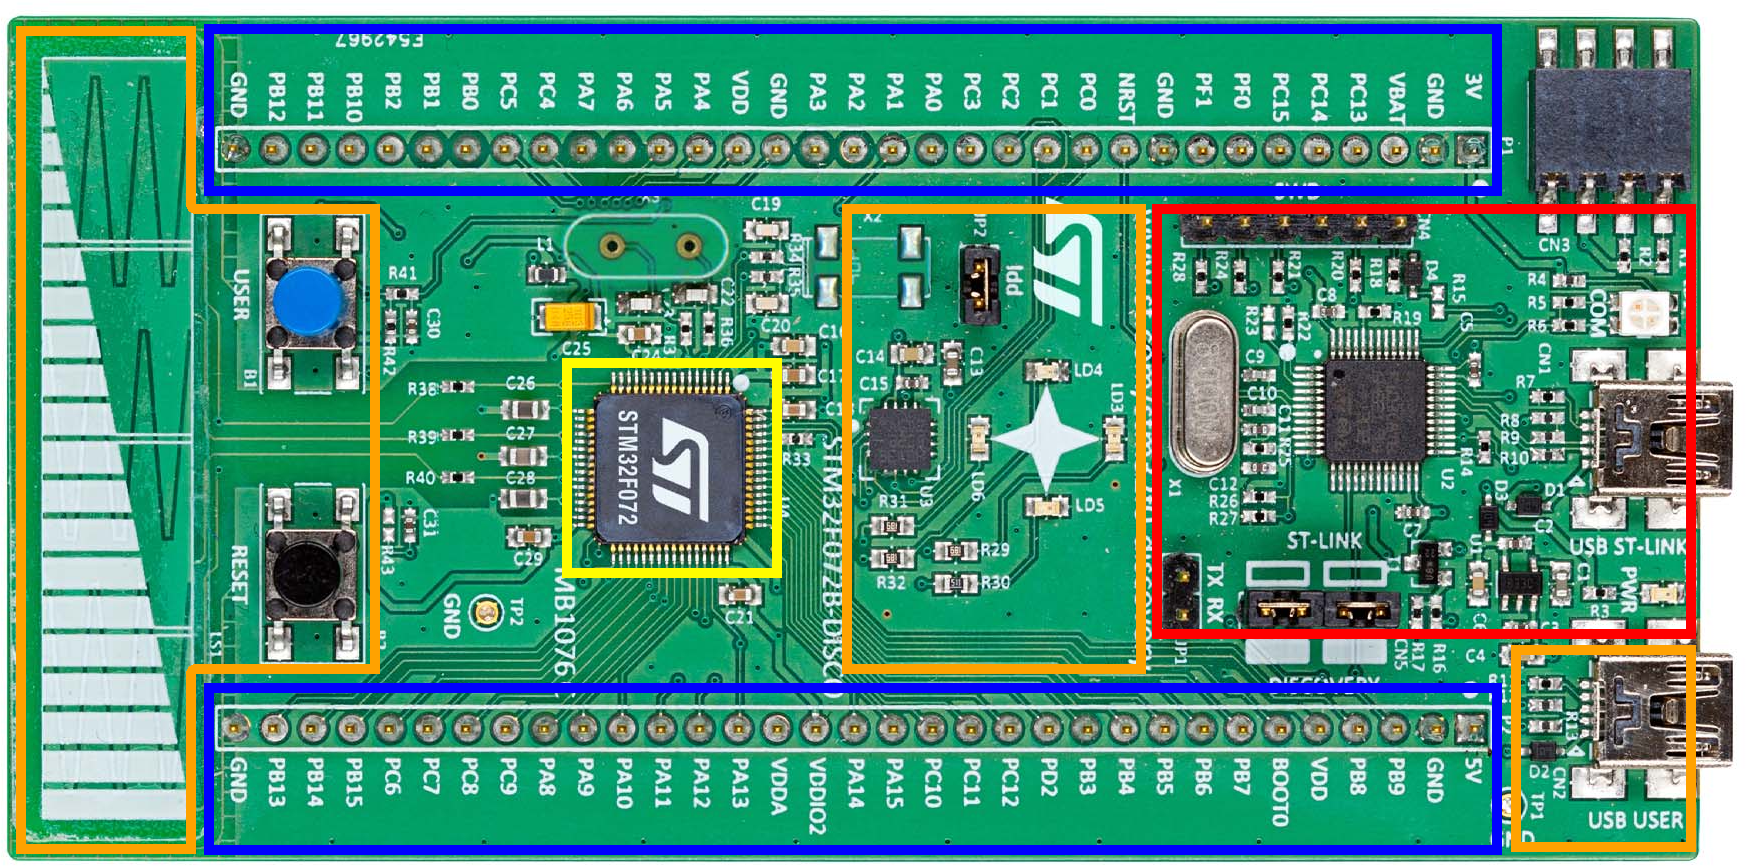
\includegraphics[width=\textwidth]{discovery_marked}
	\caption{STM32F072 Discovery Board from ST Microelectronics}
\end{figure}

% PASSIVE VOICE
One unique aspect of embedded systems programming is that the generated code is not typically run on the system used to develop the software itself. Instead, the compiled binary is loaded onto an external device for testing and debugging. Because of this, you'll be using a generic test board containing a processor and peripherals to target during development. 

The STM32F072 Discovery board is a low-cost environment which provides all of the hardware you need to start developing basic projects. There are four main parts of the Discovery board: 

\subsubsection*{STM32F072R8 ARM Cortex-M0 Processor ({\color{yellow!80!black}YELLOW})}
The STM32F072R8 features an ARM Cortex-M0 RISC core that can operate up to 48 MHz clock frequency. It has 16 Kbytes of static RAM and 64 Kbytes of Flash memory for program and data storage. It operates on voltages between 2.0 and 3.6 V and is contained in a 64-pin low-quad-flat-pack (LQFP) package. Typically these labs will use STM32F0 as a shorter name for the STM32F072R8.

The STM32F072R8 processor's name can be broken down into a couple of different parts. These parts identify the processor family, storage capabilities, and chip package the device has.

\begin{itemize}
	\item ``STM32F0'' -- Identifies the chip as a Cortex-M0 produced by ST Microelectronics
	\item ``72'' -- Specifies the device as part of the STM32F0x2 sub-family. Each sub-family has minor differences in design and peripherals offered.
	\item ``R8'' -- Indicates the FLASH (program storage) capacity and number of pins on the chip.  
\end{itemize} 

Figure \ref{f072_family} shows the entire STM32F0x2 (USB line) device sub-family. From this figure it is possible to see that there are multiple groupings of STM32F0 devices, each featuring different capabilities and containing a wide variety of parts.

\begin{figure}[]
	\centering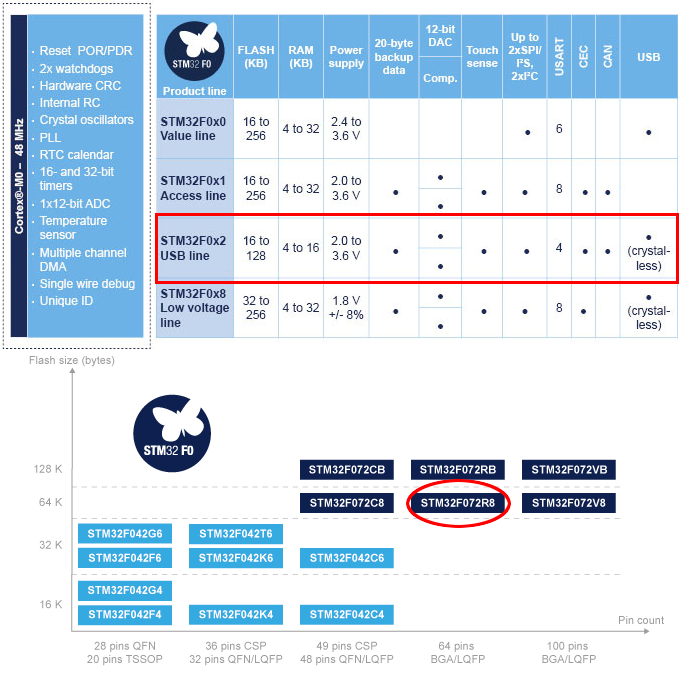
\includegraphics[width=\textwidth]{stm32f0x2_family}
	\caption{Entire STM32F0x2 device sub-family}
	\label{f072_family}
\end{figure}

\subsubsection*{ST-Link Chip Programmer and Debugger ({\color{red!90!black}RED})}
Unlike developing on many traditional systems, the STM32F0 can not communicate directly with the machine compiling the code. There are multiple methods of transferring a compiled binary to the STM32F0 (some of which can communicate directly), but the most robust method is to use a hardware debugger.

Typically many device manufacturers prefer to develop their own debugging hardware. ST Microelectronics self-developed and preferred system is known as the ST-Link. The ST-Link is itself just another ARM processor, programmed to connect via USB to the host machine. On the host machine, a number of programs can connect to the ST-Link and download a binary to the target device. The protocol spoken between the ST-Link and the STM32F0 is known as serial wire debug (SWD).  We will discuss the details of this protocol in later chapters.

\subsubsection*{Processor Breakout Pins ({\color{blue!90!black}BLUE})}	

% SPLIT INFINITIVE, PASSIVE
The Discovery board ``breaks-out'' or exposes all of the STM32F0 processor pins on the two side connectors. These make it possible to easily build and connect additional circuits to the Discovery board. The STM32F0 can control most of the pins that are available. However, there are a few occupied with system functions, such as debugging, that should not be used for other purposes. 

\subsubsection*{Experimental Hardware  ({\color{orange!90!black}ORANGE})}
Although the STM32F072 Discovery development board is simple in comparison to other development platforms, it offers a few devices for experimentation.

\begin{itemize}
	\item Light emitting diodes (LEDs) in Green, Orange, Blue and Red
	\item ``USER'' button for general purpose use
	\item ``RESET'' button
	\item Linear capacitive touch-sense bar
	\item L3GD20 3-axis MEMS Gyroscope
	\item User programmable mini-USB 2.0 port
\end{itemize}
	

\section{ARM Development Toolchain}\index{ARM Development Toolchain}

\begin{figure}[]
	\centering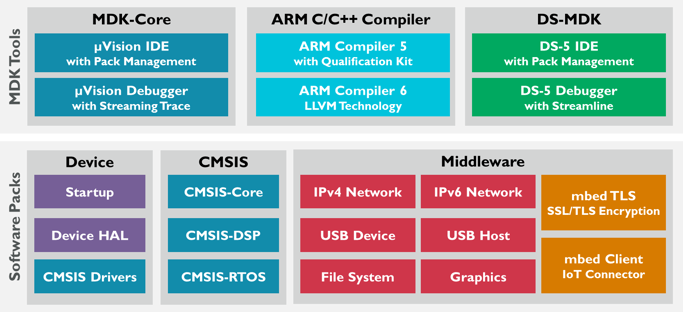
\includegraphics[width=\textwidth]{mdk_toolchain}
	\caption{MDK:ARM Toolchain}
	\label{mdk_toolchain}
\end{figure}

A \textit{toolchain} is a collection of software and hardware tools that create a complete system for developing, loading, and debugging embedded applications. 

% PASSIVE VOICE 
Figure \ref{mdk_toolchain} shows the components of the Kiel MDK:ARM toolchain. These provide a foundation for software projects and generate compiled ARM binaries. 
The toolchain can be broken into two major components, the MDK tools and supporting software packs.

\subsection*{MDK Tools}
These tools form the basis of the Kiel MDK:ARM system. The major portion that we will be using is the {\textmu}Vision IDE which targets ARM Cortex-M devices. Although not utilized in this course, the DS-MDK tools target combination processors with both application-class (Cortex-A) and embedded (Cortex-M) systems. Both IDE systems use the ARM C/C++ cross-compiler, which generates ARM/THUMB2 assembly language code.

A cross-compiler describes a system which generates assembly languages foreign from the machine that it operates on. Although the MDK:ARM system is running on a conventional PC x86-x64 architecture, it generates ARM/THUMB2 codes compatible with the Cortex-M0 STM32F0 processor.

\subsection*{Software Packs}
Similar to many conventional programming environments, embedded systems rely on supporting software libraries. 

\begin{description}
	\item[Startup Libraries] -- The STM32F0 processor requires a small amount of chip-specific initialization code to prepare the memory system and load the user application.  
	\item[Device HAL] -- The STM32F0 devices have a large number of peripherals for tasks such as timing and communication. ST Microelectronics provides files which define the bindings between these and the user application. The \textit{hardware abstraction library} (HAL), provides a C/C++ API for controlling these peripherals.
	\item[CMSIS Libraries] -- The ARM Cortex-M0 core also contains a number of advanced features. These core-peripherals are universal across all devices based on the same ARM core. The \textit{cortex microcontroller software interface standard} (CMSIS), provides a library API for interfacing with these features. 
	\item[Middleware] -- Middleware libraries provide support for higher-level functions such as file systems, USB, and graphics.
\end{description}

\section{Creating Your First Project}\index{Creating Your First Project}
Although we will be using Kiel MDK ({\textmu}Vision) to develop the software for the exercises in this book, manually creating a project for an STM32F0 processor requires a significant amount of configuration. To bypass this, we will be using the STM32CubeMX utility to graphically configure the project parameters and generate a ready-to-use {\textmu}Vision project. 

\subsection{Generating a Project in STM32CubeMX}
\subsubsection*{Selecting the Correct Processor}
\begin{wrapfigure}{L}{0.2\textwidth}
	\centering
\includegraphics[width=0.125\textwidth]{stmcube_logo}
	\caption{STM32CubeMX Logo}
\end{wrapfigure}

Launch the \textbf{STM32CubeMX (STMCube)} utility either from the start menu entry or desktop icon. Once loaded, select the \textbf{New Project} link on the welcome page, or use \textbf{File Menu \textrightarrow New Project}.

% REVISE
The \textit{New Project} window should open, here you will select the particular STM32 device that STMCube will generate a project for. The processor in use on the STM32F072 Discovery board is the STM32F072R8. You can quickly narrow down the available selections by selecting the following criteria in the \textit{MCU Filters} section.
\begin{itemize}
	\item Select \textbf{STM32F0} in the \textit{Series} filter
	\item Select \textbf{STM32F0x2} in the \textit{Lines} filter
	\item Select \textbf{LQFP64} in the \textit{Package} filter
\end{itemize}
At this point, there should only be a few choices available, select \textbf{STM32F072R8Tx} and press the \textbf{OK} button. Figure \ref{cube_newProj} shows the new project window with the appropriate filters applied.

\begin{figure}[h]
	\centering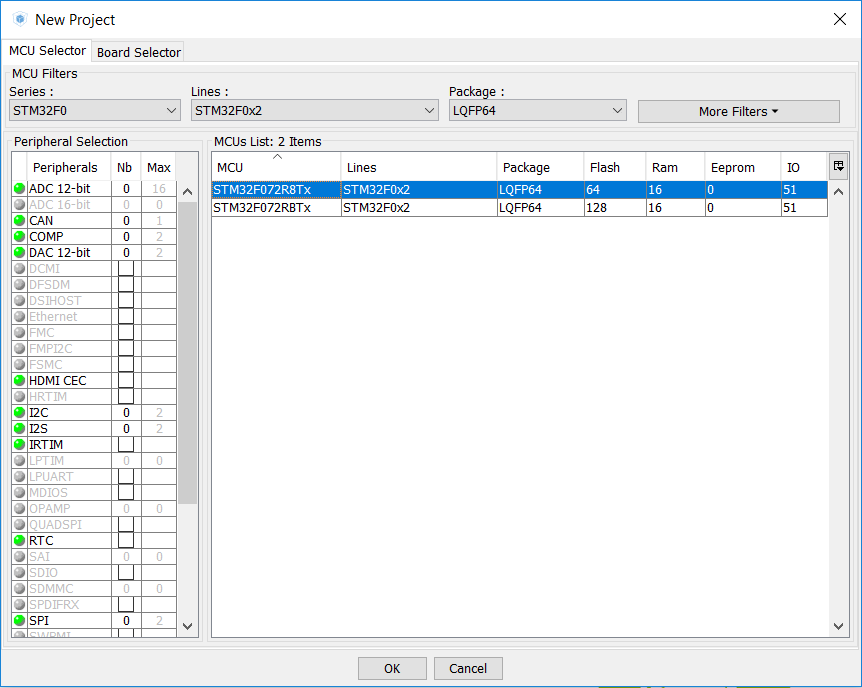
\includegraphics[width=\textwidth]{cube_newProj}
	\caption{STM32CubeMX new project window with filters applied}
	\label{cube_newProj}
\end{figure}


\subsubsection*{Changing Project Generation Settings}

% PASSIVE VOICE
After selecting the processor, you will be presented with the \textit{Pinout} screen of STMCube. (Figure \ref{cube_pinout}) This screen shows all of the available pins on the selected device and can enable and configure many of the internal peripherals within the STM32F0 processor. Although we won't be using any of the features here for this exercise, the pinout tool is very helpful for planning what pins can be used for peripheral outputs. Feel free to explore and enable peripherals on the left pane of the window but be sure to clear them all before moving on. We will be using the real capabilities of STMCube in later labs.

\begin{figure}[h!]
	\centering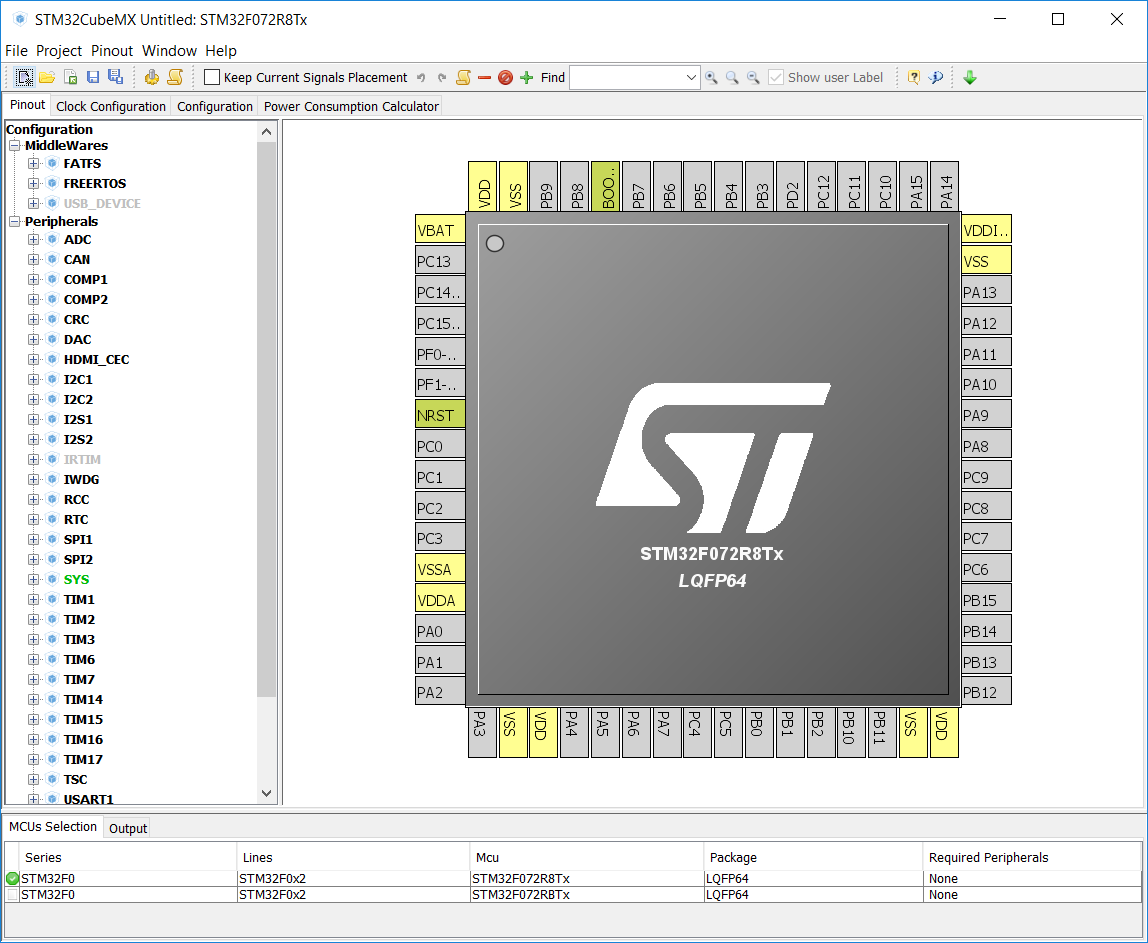
\includegraphics[width=\textwidth]{cube_pinout}
	\caption{STM32CubeMX Pinout view}
	\label{cube_pinout}
\end{figure}

Before we can tell STMCube to generate our template code project, we need to configure a few settings so that it creates the proper files and structure that {\textmu}Vision expects. To do this use \textbf{Project Menu \textrightarrow Settings}. 

Within the settings dialog shown in Figure \ref{cube_settings} you will need to configure the following attributes:
\begin{itemize}
	\item Name the new project
	\item Select a directory where STMCube can create subfolders to store project files.
	\item Change the \textit{Toolchain/IDE} dropdown menu to \textbf{MDK-ARM V5}.
\end{itemize}

%Within the settings dialog you will want to name the new project and select the directory where STMCube can create a subfolder to store project files. 
%The most important setting however is to change the Toolchain/IDE dropdown menu to "MDK-ARM V5." \\
STMCube supports a broad range of toolchains and development environments. Unfortunately, many of these are completely incompatible with each other. The Toolchain/IDE menu selects between the supported output environments and ensures that the generated project will be compatible with the IDE you are using. 

Once you are satisfied with your settings on the \textit{Project} tab, move to the \textit{Code Generator} tab at the top of the window. Although these settings are not necessarily important at the moment, you can reduce the code size of your project dramatically by selecting the \textbf{copy only the necessary library files} option in the \textit{STM32Cube Firmware Library Package} menu.
 
% PASSIVE VOICE
When the necessary project configurations have been set, close the settings dialog with the \textbf{OK} button. 

\begin{warning}
	Don't forget to set the proper toolchain in the project settings! Otherwise, it will be impossible to use the generated project files with {\textmu}Vision.
\end{warning}

\begin{figure}[h!]
	\centering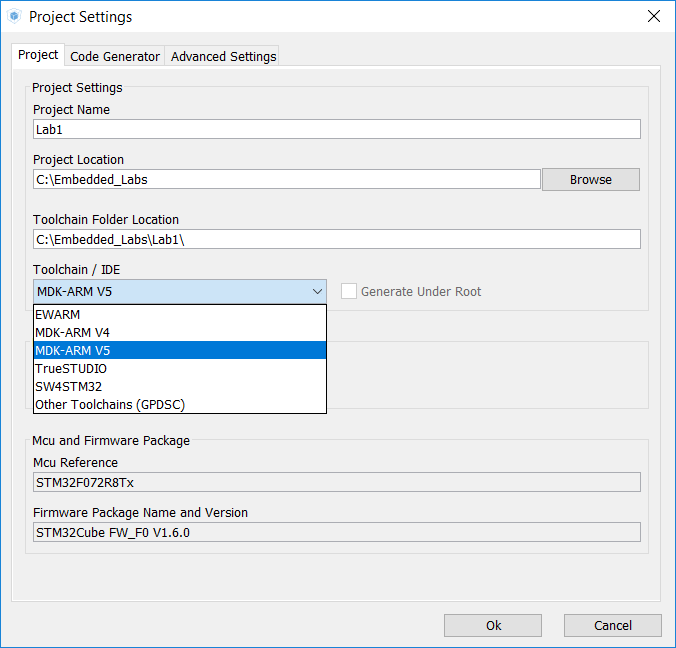
\includegraphics[width=\textwidth]{cube_settings}
	\caption{STM32CubeMX Project Settings}
	\label{cube_settings}
\end{figure}

\subsubsection*{Generating the Project}
Since we are not interested in configuring peripherals at the moment, generate the finished project using \textbf{Project Menu \textrightarrow Generate Code}. 

%PASSIVE VOICE
STMCube may take a while to copy the files to the directory specified in the settings. Afterward, you may be asked if you want to open the project folder or project file itself. You can select either of these options; we will be exploring both of them in the next section. %The next section discusses the basic directory structure of the generated Kiel MDK project. 

%\subsection{Structure of the Toolchain Project}
%Within the generated project folder there are a variety of files and subfolders. These contain {\textmu}Vision project files, startup code used to boot the STM32F0 as well as the ST Microelectronics hardware abstraction library (HAL). Within the main project directory you should find the following items:\\
%
%\begin{itemize}
%	\item \textbf{Drivers:} This folder contains support files from ST Microelectronics such as startup code and the HAL.
%	\item \textbf{Inc:} This folder contains user-developed headers, your \#include files will be placed here by {\textmu}Vision.
%	\item \textbf{MDK-ARM:} This folder holds the {\textmu}Vision project files, build metadata and compiled objects.
%	\item \textbf{Src:} This folder contains user-developed application code, .
%	\item \textbf{.mxproject \& project.ioc:} These are the STM32CubeMX project files that can be used to regenerate the project using a different configuration if needed.
%\end{itemize}


\subsection{Exploring the Project in {\textmu}Vision}

%\begin{figure}[h!]
    \begin{wrapfigure}[8]{h!R}{0.2\textwidth}
    \centering
\includegraphics[width=0.125\textwidth]{uvision_logo}
    \caption{Kiel {\textmu}Vision Logo}
    \label{uvision_logo}
    \end{wrapfigure}
%\end{figure}

Now that we have a project template that is ready to use, it is time to launch \textbf{Kiel {\textmu}Vision} from either the start menu or desktop icon and explore the development environment. 

%PASSIVE VOICE
Once {\textmu}Vision has loaded, open the newly generated project by selecting the ".uvprojx" file located under the MDK-ARM folder of the project directory. Alternatively, STMCube will also automatically launch {\textmu}Vision if the option to open the project was chosen after code generation. 

The advantage of using STMCube to generate the project is that no further configuration within {\textmu}Vision is required to start developing software. 

After the project has loaded, expand the folders within the \textit{Project} window (left-hand) of the main screen, you should see a folder hierarchy similar to Figure \ref{uvision_folders}.

\subsubsection*{Application/MDK-ARM}
% PASSIVE VOICE
This folder contains assembly-language startup code that initializes the STM32F0 processor and starts the user application after reset.  These operations depend on the particular memory map for the processor and are unique to each STM32F0 sub-family. These files are provided by ST Microelectronics and customized for Kiel's toolchain. 

\subsubsection*{Application/User}
This folder contains all user-level application code. You can find the \textit{main.c} file here, as well as any, included header files. 

If you open the physical project directory, you will find that {\textmu}Vision places c/cpp files within the \textit{Src} folder and h/hpp files within the \textit{Inc} folder. 
 
\begin{warning}
    %PASSIVE VOICE
	{\textmu}Vision chooses to list header files as sub-elements of the code that reference them. Because this project hasn't been compiled yet, you will be unable to see any of the included header files within the IDE.
\end{warning}

\begin{figure}[h!]
%\begin{wrapfigure}{R}{0.5\textwidth}
	\centering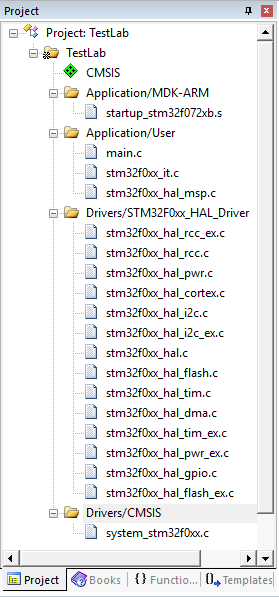
\includegraphics[width=.48\textwidth]{uvision_folders}
	\caption{Kiel {\textmu}Vision Project Structure}
	\label{uvision_folders}
%\end{wrapfigure}
\end{figure}

\subsubsection*{Drivers/STM32F0xx\_HAL\_Driver}
The STM32F0 devices are much more than a standalone processor core. Surrounding the ARM Cortex-M0 is a wide variety of peripheral circuits which connect the processor to the outside world. Similarly to the startup code, ST Microelectronics provides a hardware abstraction library. (HAL) These libraries allow the user to control system peripherals via a C-language API. %\\
%While the HAL library may be convenient to use, it does not give the user an accurate depiction of what is involved with controlling device peripherals. Because of this, we will focus on developing applications directly against the hardware interface without the use of supporting libraries.

\subsubsection*{Drivers/CMSIS}
Similar to the ST hardware abstraction library, ARM publishes a software API for the internal features of the Cortex-M0 core. These functions known as the Cortex Microcontroller Software Interface Standard, (CMSIS) provide a universal interface to all ARM devices regardless of the specific chip manufacturer. 
%This separation of processor core and device peripherals will be discussed in the next chapter. 

\subsection{Compiling and Loading a Demo Program }
\subsubsection{Auto-Generated Elements in Main.c}
% REVISE
Open the \textit{main.c} located within the Application/User folder. Within the template file, you will notice that in addition to the \texttt{main()} function there are a few others. These functions initialize the processor clock to the speed and source selected when STMCube generated the project. 

Most embedded processors have flexible clock options that allow them to run from both internal or external clock signals and operate over a wide range of frequencies. The default processor speed that STMCube configures is usually 8 MHz. If you open the STMCube files in the project directory, you can select the Clock Configuration tab and view the clock settings.

% PASSIVE VOICE
Within the main function, you will notice some automatically generated comments marking boundaries of user/auto generated code. These are used by STMCube to locate and preserve the user's code if the project is regenerated with new settings. You may decide to keep or remove these comments, but it is recommended that you manually backup changes to the \textit{main.c} file when regenerating code in STMCube regardless. 

\subsubsection{Blinky Example Code}
Figure \ref{blinky1} contains a demo program that blinks the green and orange LEDs on the Discovery board. Copy and replace the \texttt{main()} function of the template project with the contents of the example. 

%\colorbox{gray!20!white}{
%	\centering
%	\begin{minipage}{\linewidth}
%		\lstinputlisting[language=C]{./Files/blinky.c}
%	\end{minipage}
%}
%\vspace{1em}

\code{./Files/blinky.c}{Example ``blinky'' program.}{blinky1}

After replacing the main function with the ``blinky'' example, compile the project with \textbf{Project Menu \textrightarrow Build Target}. 

Kiel {\textmu}Vision uses a custom build/dependency system similar to GNU-Make to check and compile all dependencies for each application file. You can see the output from the build system in the console at the bottom of the main window.

If you generated the template project and copied the provided code correctly, you shouldn't have any errors in your completed result. Connect the STM32F072 Discovery board to the host computer using a mini-USB cable and the ST-Link USB port. 

\begin{warning}
	Remember that there are two ports available on the Discovery board. The center port is connected to the ST-Link debugger while the other is for user application use.
\end{warning}

After the Discovery board is connected, program the target STM32F0 through \textbf{Flash Menu \textrightarrow Download}. You will see a brief progress bar and status report in the {\textmu}Vision console, followed by a completion status message. 

% PASSIVE VOICE
After the loading process has completed, press and release the \textbf{RESET} button on the Discovery board. Assuming that no errors were reported in the console, you should see the orange and green lights begin to flash in an alternating pattern. \\

Congratulations, you are running a custom application on the STM32F0! 




%\section{Putting the Pieces Together}\index{Putting the Pieces Together}

%The blinky example above uses the HAL library function calls to control the ``GPIO'' or general purpose input-output peripheral. Although it might seem straightforward, there are a number of code steps required to produce something that the STM32F0 can understand. 


%%%%%%%%%%%%%%%%%%%%%%%%%%%%%%%%%%%%%%%%%%%%%%%%%%%%%%%%%%%%%%%%%%%%%%%%%%%%%%%%%%%%%%%%%%%%%%%%%
%%%%                                                                                         %%%%
%%%%       Chapter 2: Memory-Mapped Peripherals and the GPIO                                 %%%%
%%%%                                                                                         %%%%
%%%%%%%%%%%%%%%%%%%%%%%%%%%%%%%%%%%%%%%%%%%%%%%%%%%%%%%%%%%%%%%%%%%%%%%%%%%%%%%%%%%%%%%%%%%%%%%%%


\chapterimage{chapter_head_2.png} % Chapter heading image
\chapter{Memory-Mapped Peripherals and the GPIO}

\section{Overview}
This section provides an overview of embedded programs, memory-mapped peripherals, and device documentation. The exercises in this lab provide an introduction to memory-mapped register access by guiding the user through configuration of the ``GPIO'' or general purpose input-output peripheral. The GPIO is one of the fundamental peripherals available and provides access to the physical pins of the STM32F0 device. 

%\section{Explore the Processor Documentation}

\section{Basic Design of an Embedded Program}


The typical layout of an embedded program is very different from most standard programming systems. Figure \ref{programFlow} shows a comparison between devices running an operating system and the operation of many embedded applications. 
In a computer with an operating system, there are layers of supervisory code which manage low-level system operations and provide frameworks for resource sharing between multiple applications. In these systems, a user application can exit, and the operating system will continue to operate and clean up afterward. In contrast, many embedded applications execute directly on the processor core, and no operating system exists to launch or clean up after applications exit. This style of development is called ``bare-metal'' programming. 

At the beginning of every STM32F0 binary executable, there is a jump to a small region of code called the \textit{Reset Vector}. This reset vector is always executed directly after a hardware reset and is responsible for ensuring that the stack, heap, and processor clock are initialized to basic settings, allowing more complex code to operate.

Typically most of the initialization code is not within the reset vector itself but is scattered throughout the support files that ST Microelectronics and the MDK:ARM toolchain provide. The HAL library is typically used to perform less-critical initialization steps such as clock speed configuration at the beginning of the user's application. 

% PASSIVE VOICE, REVISE
After device initialization, the startup code calls the \texttt{main()} function within the user's application. Typically, embedded programs begin by configuring hardware peripherals they require and then enter into an infinite loop containing the majority of the application. This endless loop is always required since the main function of an embedded program should never return. Unlike a machine with an operating system, there is nothing to catch the processor's execution after the main program exits. This means that the behavior of the processor after returning is undefined and could range from resetting the device to executing random data.

\begin{figure}[]
    \centering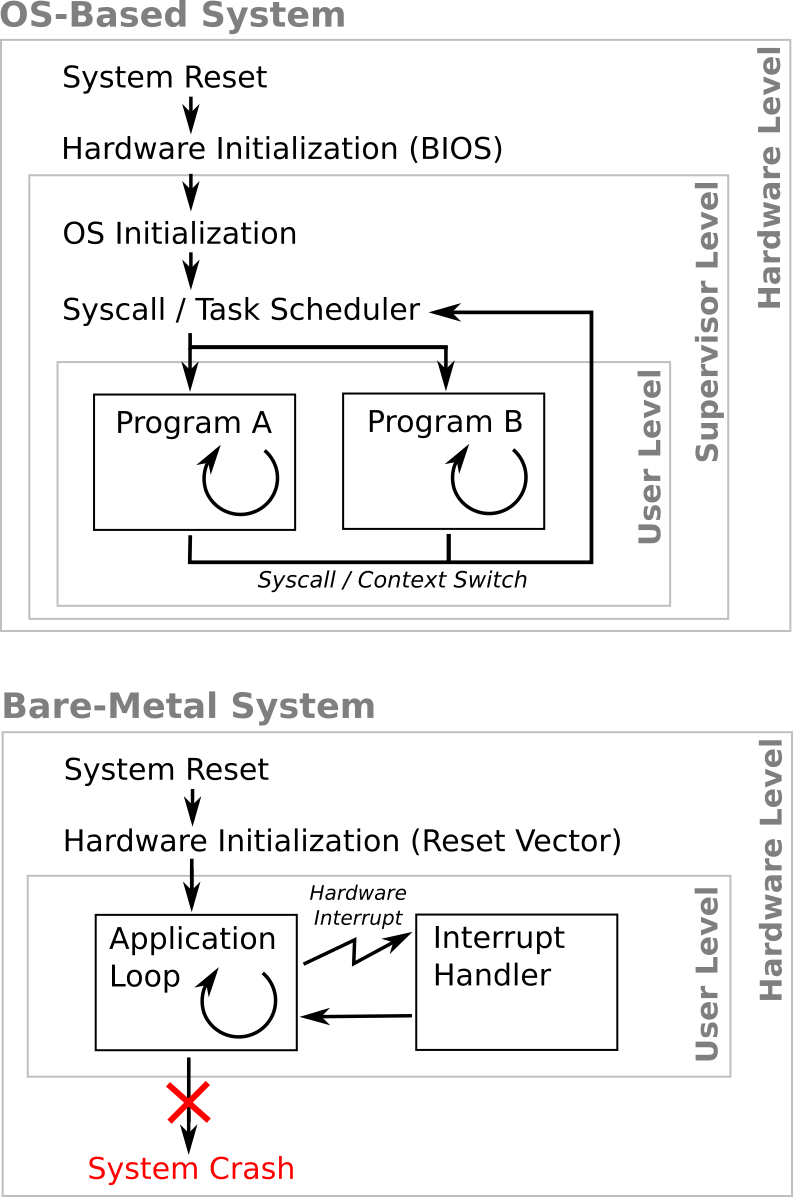
\includegraphics[width=.75\textwidth]{programFlow}
    \caption{Comparison of operating-system and bare-metal systems. }
    \label{programFlow}
\end{figure}


\section{Controlling Device Peripherals}

The last lab section introduced the ``blinky'' example program. (shown in Figure \ref{blinky}) This simple program repeatedly toggles pins on the STM32F0 using the GPIO hardware abstraction library drivers. This results in a pattern of alternating flashes as the pins used, connect to LEDs on the STM32F072 Discovery board. 
%\code{./Files/blinky.c}
\code{./Files/blinky.c}{Example ``blinky'' program.}{blinky}

Taking a closer look at the program structure shows that it begins by initializing the HAL library and system clock. Afterward, it initializes the specific GPIO peripheral controlling the desired pins and enters an infinite \texttt{while} loop. Although many of the function calls in this example program are relatively straightforward to understand, an important question to consider is how the HAL library functions modify the physical peripherals of the STM32F0 device.

\subsection{Memory-Mapped Peripherals on the STM32F0}

\begin{figure}[]
    \centering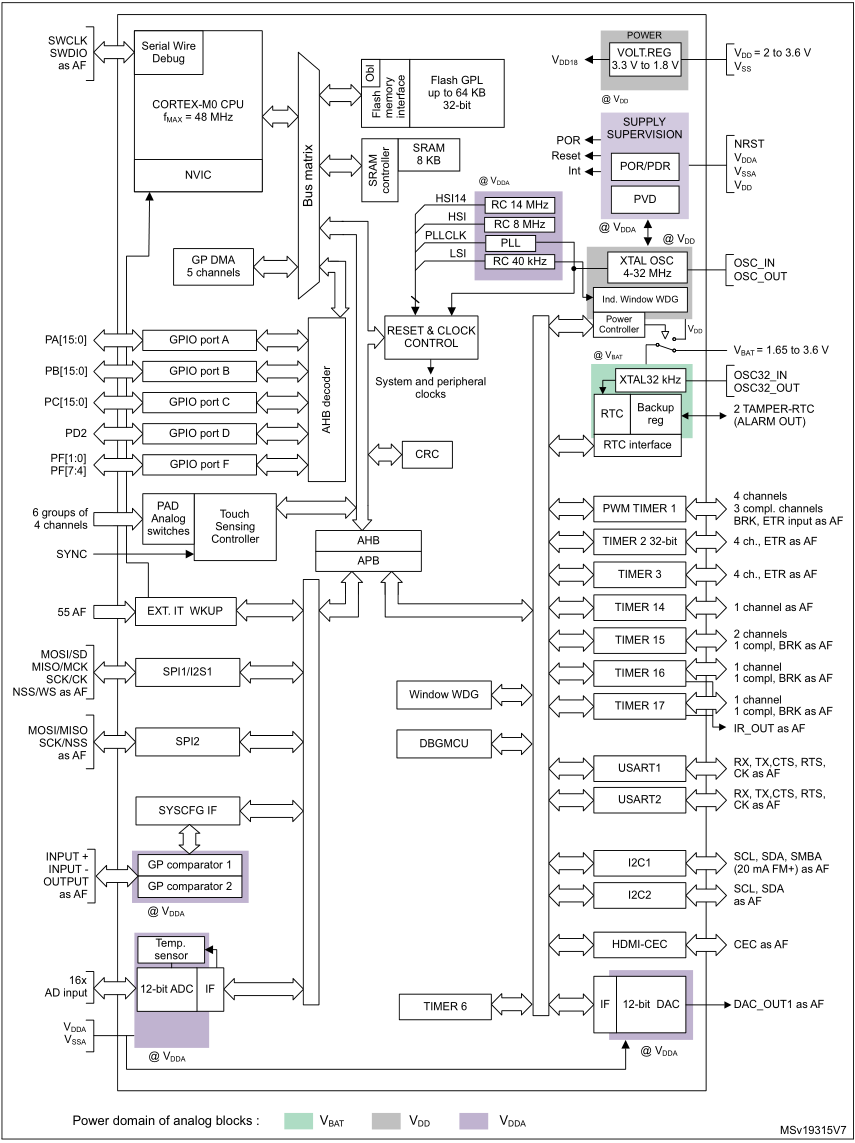
\includegraphics[width=\textwidth]{peripherals}
    \caption{Peripheral block diagram for the STM32F0 devices}
    \label{peripherals}
\end{figure}

Figure \ref{peripherals} contains the system block diagram for the STM32F0 family of processors. As shown, there are an enormous number of peripherals available, and the interconnections between them are complex. Luckily, the toolchain hides most of the complicated hardware-level implementation from the end user.

However, how does the processor interact with the complex hardware surrounding it? There are many methods that an engineer can choose when designing a processor core. One of these is to develop the machine language interface so that it understands specific instructions telling it to manipulate the hardware in a certain way. This method seems straightforward but has the disadvantage of increasing the size and complexity of the instruction decoder hardware. Likewise, if the processor has a significant number of peripherals, the resulting instruction set becomes enormous. 

ARM processors belong to the \textit{reduced-instruction-set-computing} (RISC) class of devices. Processors of this type have instruction sets that are relatively simple and typically perform a limited number of tasks. Usually, these tasks/instructions primarily involve arithmetic operations and moving data around the system's memory.

% PASSIVE VOICE
Because of this limitation, one of the most common ways of controlling system hardware is to designate regions of memory as \textit{peripheral registers}. When an application writes to the memory address of one of these registers, the memory bus controller recognizes the address as belonging to a specific peripheral. It then routes the data to the appropriate control circuitry for that peripheral instead of system memory. Because these hardware registers are mapped into the system's memory address space, the processor simply considers them as conventional variables. 

Figure \ref{memoryTable} shows a simplified memory map for a STM32F0 processor. Although the STM32F0 devices have only a few kilobytes of combined physical memory, program storage, and mapped peripheral registers, they have a full 32-bit (4GB) address space. Because of this, huge blocks of unimplemented addresses separate each functional region of the address space (program storage, physical memory, and peripheral registers). These gaps in the address space ensure that each type of memory has a unique-bit-pattern and provides for future expansion when developing new chips. 

\begin{figure}[]
    \centering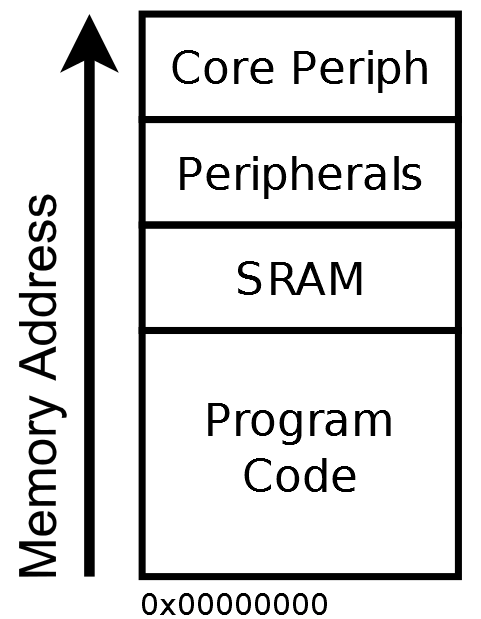
\includegraphics[width=0.25\textwidth]{memoryTable}
    \caption{Simplified memory table for STM32F0 devices.}
    \label{memoryTable}
\end{figure}


\subsection{Differences Between ARM-Core and Device Peripherals}

One unique feature of all ARM chips is that the processor core is developed separately from the rest of the device. ARM Ltd. develops the Cortex processors and licenses the designs to hardware manufacturers to implement into real systems. 

%PASSIVE VOICE
Since the processor core is developed separately, it contains its own set of peripherals. These peripherals have a much closer relationship to the operation of the processor and involve actions that directly manipulate the flow of instruction execution. Examples of these include hardware interrupts and program debugging. Because core peripherals are physically separate from the others within the device, they are memory mapped within a separate region. However, the biggest difference to system programmers is that these peripherals are documented separately from the others.

\section{Searching Datasheets and Manuals for Peripheral Details}

Efficiently searching datasheets and manuals is one of the most important skills that an embedded engineer can develop. This trait is important because the sheer amount of information required to understand the operation of many embedded devices completely is staggering. 
Engineers who can rapidly search for information within device documentation do not need to memorize operation details. Likewise, it becomes easier to work with an unknown device. 

Four files provide the documentation for the exercises in these labs. You can download these from the following links. However, it is always a good idea to know how to find them on a manufacturers website.

\begin{enumerate}
    \item \href{http://www.st.com/content/ccc/resource/technical/document/datasheet/cd/46/43/83/22/d3/40/c8/DM00090510.pdf/files/DM00090510.pdf/jcr:content/translations/en.DM00090510.pdf}{\textbf{(STM32F072RBT6 Datasheet) DM00090510.pdf}}
    \begin{itemize}
        % REVISE
        \item The chip datasheet provides device-specific details for the processor used. This includes pin connections for available chip packages and a list of available peripherals.
    \end{itemize}
    \item
    \href{http://www.st.com/content/ccc/resource/technical/document/programming_manual/fc/90/c7/17/a1/44/43/89/DM00051352.pdf/files/DM00051352.pdf/jcr:content/translations/en.DM00051352.pdf}{\textbf{(Programming \& Core Manual) DM00051352.pdf}}
    \begin{itemize}
        \item The core programming manual gives us information on the ARM-core peripherals as well as the assembly instruction set. It is generic to all of the processors within the STM32F0 family.
    \end{itemize}
    \item
    \href{http://www.st.com/content/ccc/resource/technical/document/reference_manual/c2/f8/8a/f2/18/e6/43/96/DM00031936.pdf/files/DM00031936.pdf/jcr:content/translations/en.DM00031936.pdf}{\textbf{(Peripheral Manual) DM00031936.pdf}}
    \begin{itemize}
        \item The peripheral reference manual contains detailed information on all peripherals that can be made available within an STM32F0 device. However, not all STM32F0 devices contain every peripheral! The chip datasheet is required to determine which peripherals are available for use.
    \end{itemize}
    \item 
    \href{http://www.st.com/content/ccc/resource/technical/document/user_manual/3b/8d/46/57/b7/a9/49/b4/DM00099401.pdf/files/DM00099401.pdf/jcr:content/translations/en.DM00099401.pdf}{\textbf{(Discovery Board Manual) DM00099401.pdf}}
    \begin{itemize}
        \item The Discovery board manual contains schematics and tables, showing the onboard devices and connectors attached to the STM32F0. The Discovery board silkscreen also documents many device connections. 
    \end{itemize}
\end{enumerate}

\begin{warning}
    These manuals are large! Do not expect to read them fully; there is simply too much information presented. For example, the peripheral reference manual contains over 1000 pages of detailed descriptions about each peripherals operation and configuration.
\end{warning}

\subsection{An Example: The General Purpose Input-Output Peripheral (GPIO)}


The GPIO is one of the most fundamental peripherals within the STM32F0. Although it is one of the simplest peripherals, it is still surprisingly complex and very powerful.

% PASSIVE VOICE
Open the STM32F0 peripheral reference manual to page 156; this should be the heading ``General-purpose I/Os (GPIO).'' The reference manual is sectioned by bookmark links, if the PDF viewer used can show these (see Figure \ref{bookmarks}) they can be used to navigate to desired sections quickly.

\begin{figure}[]
    \centering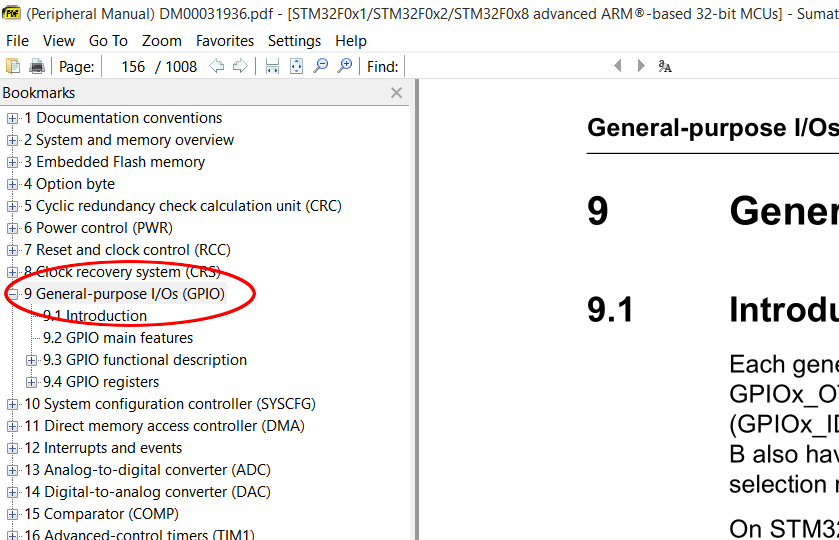
\includegraphics[width=\textwidth]{bookmarks}
    \caption{Navigation bookmarks in the peripheral reference manual.}
    \label{bookmarks}
\end{figure}

Each section of the reference manual is organized such that it first introduces the available features and modes of the peripheral. Afterward, it explains in detail the operation of the different modes,  including graphs, figures, and tables showing characteristics of the peripheral's operation. Finally, it provides detailed explanations of each user-accessible control register that configures the peripheral.

% REVISE
To understand the GPIO control registers, it is helpful to discuss the different modes it can operate in. Go back to page 156 in the reference manual (beginning of GPIO section) and look through the information on that page.

The \textit{GPIO main features} section indicates that a GPIO pin can have the following modes:

\begin{itemize}
    \item Output Configuration
    \begin{itemize}
        \item Push-Pull -- Pin is pushed to Vcc when logic `1', pulled to GND when logic `0.'
        \item Open-Drain -- Pin can only be pulled to GND when logic `0', floats when logic `1.'
    \end{itemize}
    \item Digital Input Configuration
    \begin{itemize}
        \item Floating -- Pin has high-impedance, voltage ``floats'' unless externally pulled to a state.
        \item Internal Pull-Up/Down -- Pin has internal ``resistor'' to Vcc or GND.
    \end{itemize}
    \item Analog Input Configuration
    \begin{itemize}
        \item Pin is connected to the system analog peripherals instead of a digital comparator.
    \end{itemize}
    \item Alternate Function Configuration
    \begin{itemize}
        \item Pin is connected to a selection of internal peripherals. These directly control the pin operation.
    \end{itemize}
\end{itemize} 

Additionally, there are other features such as configurable speed, register locking, bit-set-reset and more. This lab section only considers two basic configurations: push-pull output and floating input.

% REVISE
Begin by examining the configuration registers within the GPIO peripheral. Beginning on page 165, the manual starts with the most important register of them all. 

\subsubsection{GPIO Port Mode Register (GPIOx\_MODER)}

The port mode is the most important register in the GPIO peripheral. Without configuring this register, it is impossible to use GPIO pins as anything aside from digital inputs. Examining the register map in the manual shows a table of 16 cells titled ``MODER0[1:0]'' through ``MODER15[1:0]''. Notice that above these cells are numbers ranging from 0-31 and below are cells with ``rw'' in them. Breaking these down gives the following explanations: 

\begin{itemize}
    \item The STM32F0 processors have multiple GPIO peripherals known as \textit{ports}, these are named in the following manner: GPIOA, GPIOB ... GPIOx. Within a GPIO port, there can be up to 16 pins; these pins are named in the following manner: PA0 (GPIOA, Pin 0) ... PA15 (GPIOA, Pin 15), PB0 (GPIOB, Pin 0) ... etc.
    % PASSIVE VOICE, REVISE
    \item STM32F0 devices do not recognize inputs/outputs on a chip by physical pin numbering. The reason for this is because different chip packages have differing numbers of pins, and the pin ordering between these is inconsistent. GPIO pins are instead labeled with a port name (PA0 for example) which describes where to go to configure it. Within the chip datasheet, there is a table mapping GPIO pin names to physical pin numbers on the specific chip package used.
    \item Since there can be up to 16 pins in a GPIO bank, there are 16 ``MODER'' cells (pairs of bits) within the mode register. Because GPIO pins start counting from 0, the 16 pins are numbered 0 through 15.
    % PASSIVE VOICE, REVISE
    \item The number above each cell in the register map indicates the bit number within the register. Each ``MODER'' cell consists of 2 bits; this is because there are four main modes that pins can be configured into. A description of the different modes, as well as the bit patterns, used to select them, are directly below the register map.
    To choose one of these modes, the bits within the correct ``MODER,'' cell for the desired pin must be set to the corresponding bit pattern.
    \item The ``rw'' below each of the cells in the register map indicate that the corresponding bit can be both read and written. Sometimes individual bits or entire registers are read-only or write-only.
\end{itemize}

\begin{example}[Setting a Pin to Output Mode]
    The following steps configure pin PB3 to be an output. Figure \ref{modeReg} outlines these using the GPIOx\_MODER register map in the peripheral reference manual.
    \begin{enumerate}
        \item The name PB3 indicates that the pin belongs to the GPIOB peripheral and is the fourth pin in the control register. (pin numbering begins at zero)
        \item The fourth cell in the GPIOx\_MODER register map is labeled ``MODER3'' and contains bits 6-7.
        \item Examine the bit patterns listed below the register map. One of these \{\texttt{01}\} corresponds to ``General purpose output mode.''
        % PASSIVE VOICE
        \item The output mode bit pattern indicates that for the two configuration bits, the lower should be set to `1' and the upper should be cleared to `0'.
        \item Since bits 6-7 in the GPIOx\_MODER register control pin PB3, setting bit 6 and clearing bit 7 will configure the pin to output mode. 
    \end{enumerate}  
\end{example}

\begin{figure}[]
    \centering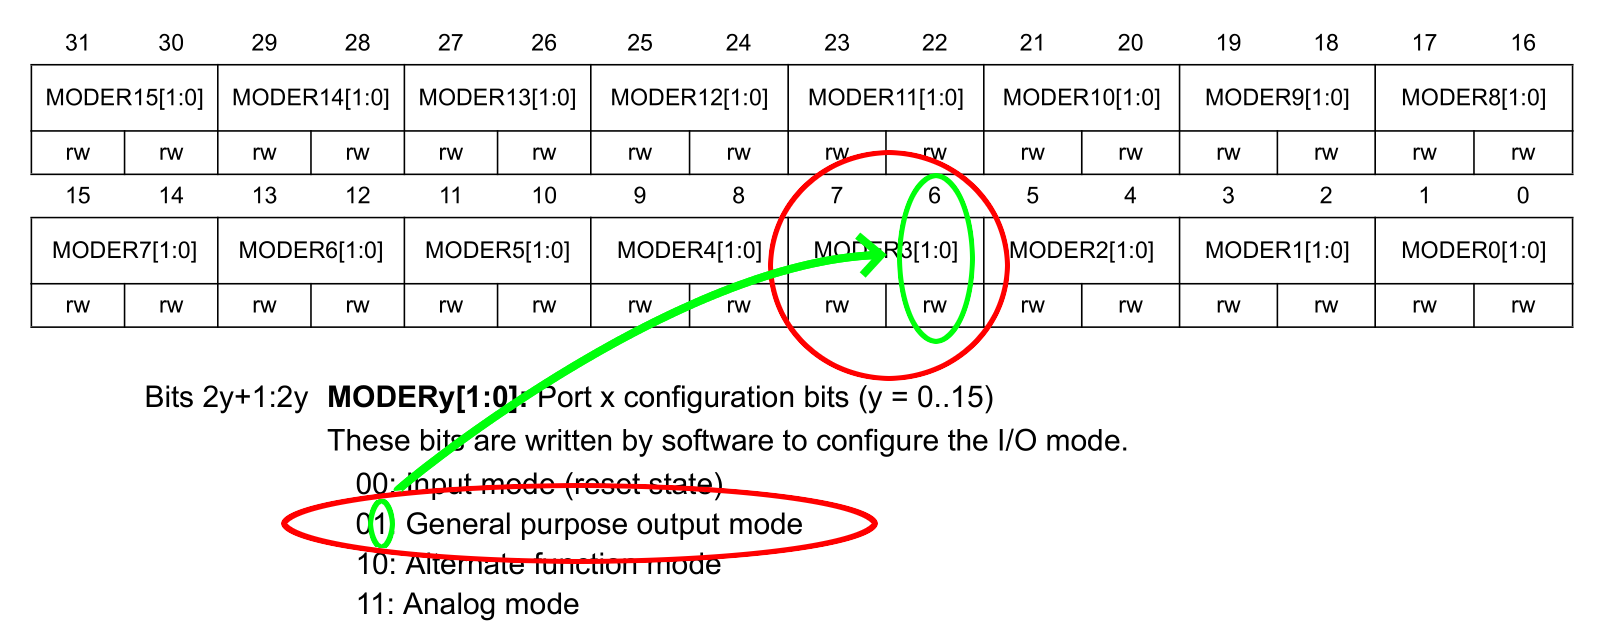
\includegraphics[width=\textwidth]{modeReg}
    \caption{Configuring the mode register to set a pin to output mode.}
    \label{modeReg}
\end{figure}

\subsubsection{GPIO port output type register (GPIOx\_OTYPER)}
% PASSIVE VOICE
This register selects what type of output mode you want for each pin configured as an output. For pins that aren't configured in output mode, the bits in this register have no effect. Since there are only two possible modes, there is only one bit per pin defined. The rest of the register is ``reserved'' and you shouldn't try to write anything there.

\subsubsection{GPIO port output speed register (GPIOx\_OSPEEDR)}
% PASSIVE 
One of the major selling points of ARM processors is that they typically use very low power. One way that they manage to reach such low power consumption is because most peripherals are either disabled and/or slowed-down by default. GPIO pins on an STM32F0 can be configured into three different speed modes, with the slowest using the least amount of power and the fastest using the most.

% REVISE
You might notice that the reference manual does not tell you how fast each speed mode operates. This is because it is dependent on the specific STM32F0 processor used. You can find out the different speed modes by looking in the device datasheet, section 6.3.14 (Electrical characteristics \textrightarrow Operating conditions \textrightarrow I/O port characteristics \textrightarrow I/O AC characteristics).

\subsubsection{GPIO port pull-up/pull-down register (GPIOx\_PUPDR)}
This register connects internal pull-up or pull-down ``resistors'' to a pin. These resistors are actually transistors that are not completely turned on but will leak enough current to act as a high-value resistor. (>100kOhm usually) Typically the internal pull resistors are only used for input modes.

% REVISE
One thing to notice with the option bits for this register is that one of the bit patterns is reserved. This means that you should never set the bit-pairs in the register into that state, although undefined it is possible that it could turn on both the pull-up and the pull-down resistors and waste power.

\subsubsection{GPIO port input data register (GPIOx\_IDR)}
All of the registers that we've seen so far have been read-write, we can both read and write to them to modify pin configuration. If you look at the register map, you'll find that all the bits in this register are read-only.

% PASSIVE
The data input register always shows the logical state of each pin in the GPIO port. If the pin is an input, then the matching bit will show whatever logical state the outside world is driving that pin. If a pin is configured as an output, then it will show whatever logical state you have set that pin to be with the output register.

\subsubsection{GPIO port output data register (GPIOx\_ODR)}
This register sets the logical state of pins configured to be outputs. If you write a `0' to a bit in this register, then its matching pin will be pulled low. If you write a `1' to the bit, then the pin will be driven high.

\subsubsection{GPIO port bit set/reset register (GPIOx\_BSRR)}
This register is write-only. The reason why is that it's a shortcut to set and clear bits in the output register. Typically you can't just overwrite an entire register with a new value for a single bit because there are other bits that you don't want to overwrite. You first have to read the register value, perform a bitwise operation, so the bit you want is modified and then write it back.

The bit set/reset register allows for much faster modification of the output register because you never have to read or worry about other bits except the one you want to modify. You can simply overwrite the entire register; it will only modify the output register on the bits you have set.The lower half of this register sets bits in the output, the upper half clears/resets them.

\subsubsection{GPIO port configuration lock register (GPIOx\_LCKR)}
% REVISE
The configuration lock register locks the other configuration registers for the associated pin. It's intended to prevent a malfunctioning program from accidentally changing a pin into an unwanted mode. Once the lock is activated, you can't edit the lock register unless you first go through a timed sequence of writes on a specific bit. This is an advanced feature that you typically won't use often.

\subsubsection{GPIO alternate function low/high registers (GPIOx\_AFRL/GPIOx\_AFRH)}
% PASSIVE, REVISE
Looking at these registers you'll notice that every pin has four bits for configuration. This means that there are two 32-bit registers (AFRL \& AFRH) needed to configure alternate functions for all 16 pins. The alternate functions that each pin can be connected to depends on the specific processor and pin. There is a table in the device specific datasheet which lists the possible alternate functions for each pin, as well as what number each function has.

We will be using alternate functions in the next lab to connect GPIO pins to timer peripherals.

\subsubsection{GPIO port bit reset register (GPIOx\_BRR)}
This last control register in the GPIO peripheral is very similar to the bit set/reset register. Although you can clear bits using the bit set/reset register, all of the clearing bits are in the upper half of the register. This reset-only register is essentially a copy but has the clearing bits in the lower half. If you look at the mapping between bits in this and the bit set/reset register and their effect on the output register you might see why some people wanted the clear bits also in the low positions.

\subsection{Finding What Peripherals are Available in a Device}

Sometimes the peripheral reference manual can be misleading because it documents all peripherals that can appear on any of the STM32F0 devices. However, depending on which member of the STM32F0 family you have it's unlikely that every documented peripheral is available.

You can discover what peripherals each specific device features by examining the first few pages of the chip datasheet. These pages contain a summarization of available peripherals. However, they don't usually give important details about the features and limitations these may have. 

% PASSIVE
Within the \textit{Functional Overview} (Section 3) of the datasheet, you will find more details about the peripherals that are included within the specific chip. 

\begin{example}[System Timers and their Features]
    % PASSIVE
    Examine the first page of the STM32F072RB datasheet. Within the section discussing the \textit{timer} peripherals, notice that while the basic type of the timers (16 or 32-bit) are listed, no real details of their capabilities are given. 
    
    Afterward, turn to page 21 of the STM32F072RB datasheet. Here the functional overview contains the table shown in figure \ref{timers}. This table lists the individual characteristics and names of the available hardware timers.
\end{example}


%STM32F072RB
\begin{figure}[]
    \centering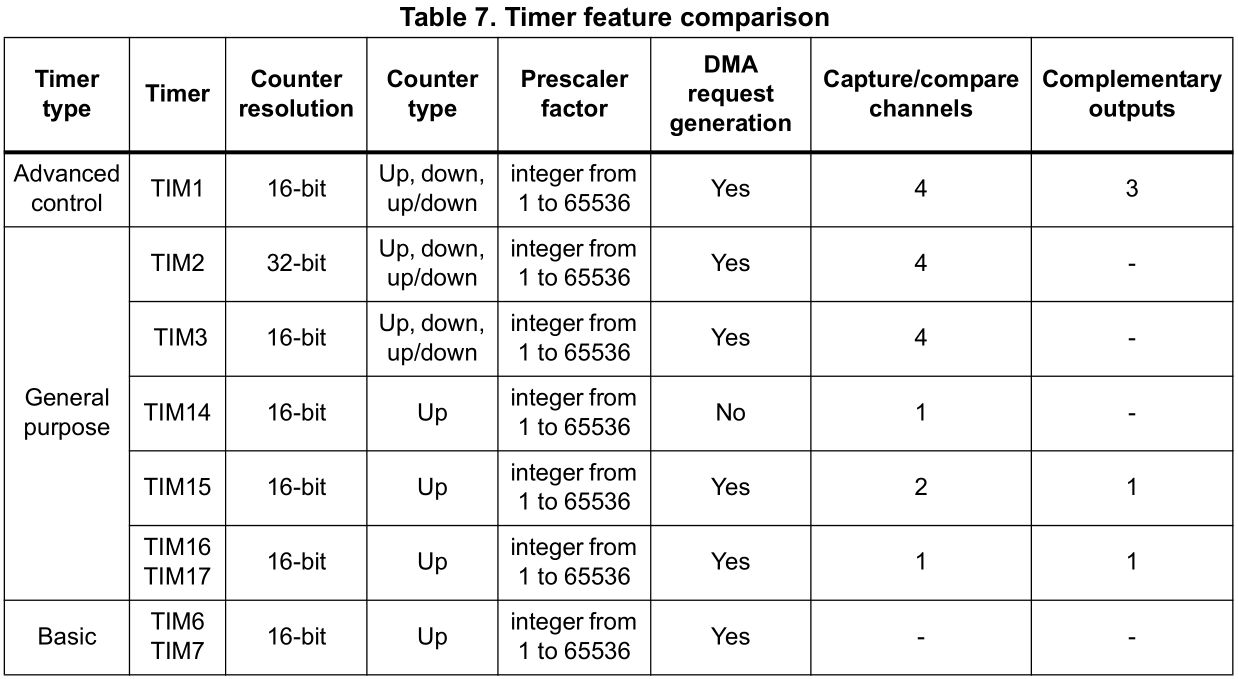
\includegraphics[width=\textwidth]{timers}
    \caption{STM32F072RB hardware timer details}
    \label{timers}
\end{figure}

\subsection{Finding Register Definitions in ST's Header Files}

Take a look at the following line of code; you'll notice that I'm casting a hexadecimal memory address to a pointer, dereferencing that pointer and writing data to the memory location that the dereferenced pointer references. This code accesses the GPIOC mode register (GPIOC\_MODER) and configures pins PC8 and PC9 to output mode.

\ilcode{*((volatile uint32\_t*) 0x48000800) = 0x50000;}%{0.25em}
\smallskip
%\texttt{*((volatile uint32\_t*) 0x48000800) = 0x50000;}\\

% REVISE
While pointers and memory addresses are technically the only method available to interact with peripheral registers, the pointer cast and dereference syntax is not particularly convenient.

%REVISE
Although most embedded code simplifies into statements like this, we do not typically have to look up memory addresses and make/dereference pointers as previously shown. This is because ST provides header files which name and organize hardware registers into structures that are reasonable to deal with. Using these header files, the pointer code above becomes much simpler as shown below.

\ilcode{GPIOC->MODER = 0x50000;}%{0.25em}
\smallskip

%\texttt{GPIOC->MODER = 0x50000;}\\

% PASSIVE
Looking back to the GPIO register pages in the peripheral reference manual, you will notice that each register has been given a short abbreviated name. Likewise you will see that the bits within the registers are also named. Figure \ref{regName} shows the highlighted names for the GPIO mode register. 

\begin{figure}[]
    \centering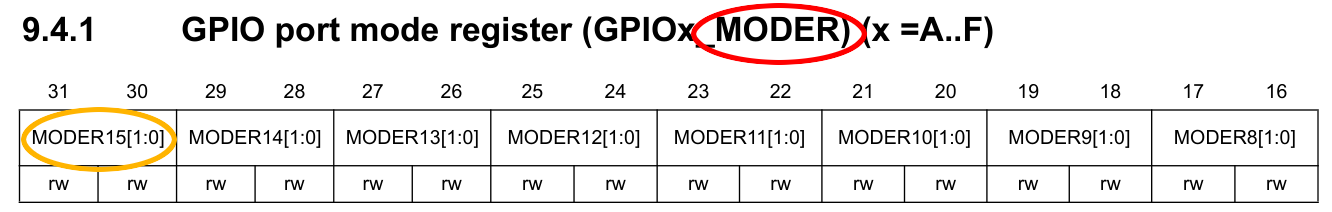
\includegraphics[width=\textwidth]{regName}
    \caption{GPIO mode register with keyword names circled}
    \label{regName}
\end{figure}

% PASSIVE
A good question to ask at this point would be where the names for registers are defined, and how they are accessed from a C program? The answer is within the \textit{CMSIS Cortex-M0 Device Peripheral Access Layer Header Files} also known as ``stm32f0xx.h'' and its derivatives. Originally all peripheral information for the entire STM32F0 line was defined in ``stm32f0xx.h''. However, in recent versions of the HAL, ST Microelectronics has split the information for each device sub-family into separate files. 

Open a {\textmu}Vision project and expand the project hierarchy under ``main.c.'' If {\textmu}Vision doesn't show any included headers after expanding the hierarchy, compile the project, and it should update after parsing the code dependencies. Within the list of these files, you should see the both ``stm32f0xx.h'' and ``stm32f072xb.h.''  Alternatively, you can locate these files manually by searching for them within the project directory under: "Drivers\textbackslash CMSIS\textbackslash Device\textbackslash ST\textbackslash STM32F0xx\textbackslash Include." 

\subsubsection{Searching the ``stm32f072xb.h'' File}

Open the ``stm32f072xb.h.'' file and look for the introductory header comment which gives a summary of the functionality provided. Since many IDE's like to collapse large sections of commented text you may need to expand the comment with the small ``+'' icon near the line numbers. Because the "stm32f072xb.h" file is large (>10000 lines) you will need to use the text search features of the IDE to navigate. In order to do this, we need to get familiar with how the file organizes peripherals and their registers

Move down to line 390; you will notice that this is a typedef for a C-structure representing a GPIO peripheral. This structure type creates a neat package for named pointers to each of the control registers a GPIO peripheral has. Because this code is a c-type definition, the system can create named copies of the structure for every GPIO peripheral in the device. The "stm32f072xb.h" file also defines the contents of the register pointers in each peripheral structure, so we don't need to deal directly with memory addresses.

\begin{figure}[]
    \centering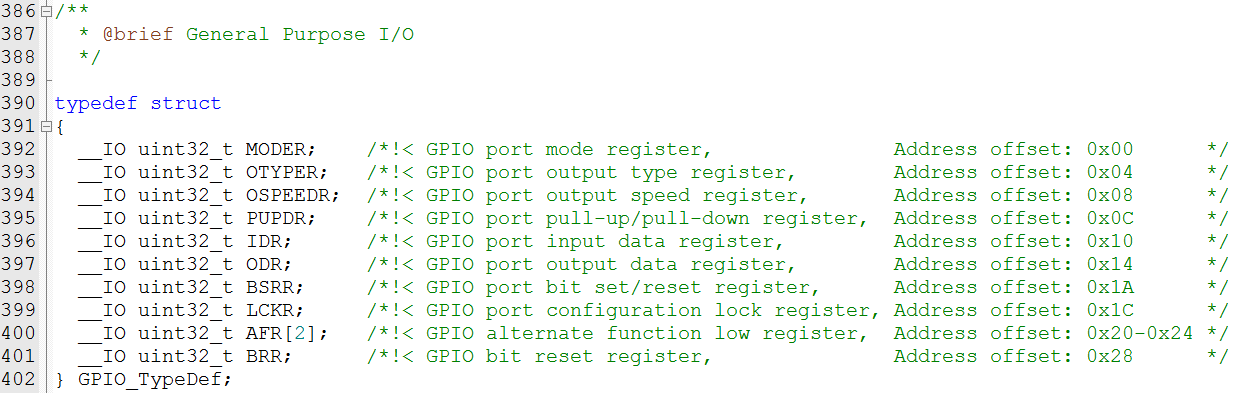
\includegraphics[width=\textwidth]{struct}
    \caption{GPIO structure definition}
    \label{struct}
\end{figure}

Returning to the top of the header file, open {\textmu}Vision's text search feature by selecting: \textbf{Edit Menu \textrightarrow Find}. Type ``GPIO'' into the search box and hit the find button. More likely than not, {\textmu}Vision's took you directly to line 390 again. Typically, searching on a guess of the peripheral name is the easiest way to start finding the documentation you'll need. Now, open the text search window again and search for the structure name defining the GPIO peripheral, you'll find it right after the closing curly-brace at the end of the GPIO structure code. ("GPIO\_TypeDef")

Searching on the name of the GPIO structure likely took you to line 785. Here we can see the multiple named copies of the GPIO structure, one for each of the physical GPIO peripherals within the STM32F0 chip. These define statements show the actual name you will use to access the structure for that peripheral.

Returning again to the structure definition, (line 390) try searching on one of the register names it defines. If you searched on the MODER register, you will find that eclipse took you to line 6499 where a list of defines gives names to each of the bits in the register. For simple peripherals like the GPIO, we typically won't use the bit names since their purpose is fairly straightforward and all have similar functions (just on different pins). For more complex peripherals the bit names often tell you their function, we'll see an example of this later.


\section{Starting to Write Embedded Programs}

If you've made it this far, you're almost ready to start writing your own embedded applications. There's just a few thing you need to know before your code will work properly.


\subsection{Bitwise Operations on Peripheral Registers}

This lab assumes that you have had prior experience with \textit{bitwise} logic operations. Because of this, we'll just have a rapid overview of common tasks. Bitwise logic allows us to manipulate portions of a register without overwriting the rest.

\subsubsection{Setting bits}
To set bits in a register, bitwise-OR its value with a bitmask. Any bits set in the bitmask will be applied to the register's value. The bitwise-OR operator is a single vertical-pipe character `|.'

\ilcode{GPIOC->MODER |= 0b00001000;    // Sets the 3rd bit}%{0em}

\subsubsection{Clearing bits}
% PASSIVE
To clear bits in a register, bitwise-AND its value with a bitwise-Inverted bitmask. Any bits set in the bitmask will be cleared from the register's value. The bitwise-AND operator is a single ampersand character `\&', the bitwise-Invert is the tilde character `\textasciitilde.'

\ilcode{GPIOC->MODER \&= ~(0b00001000);    // Clears the 3rd bit}%{0em}

\subsubsection{Inverting/Toggling bits}
Although there is a bitwise-Invert operator `\textasciitilde' it inverts every bit in the target. To selectively invert a few bits in a register, bitwise-XOR its value with a bitmask. Any bits set in the bitmask will cause the matching bit in the register's value to be inverted. The bitwise-XOR operator is a single caret character `\textasciicircum.'

\ilcode{GPIOC->MODER ^= 0b00001000;    // Inverts the 3rd bit}%{0em}

\begin{warning}
    % PASSIVE
    Note that {\textmu}Vision does \textbf{not} allow binary constants with the ``\texttt{0b}'' prefix. The binary constants shown here are used only for clarity. Within the actual code, hexadecimal constants with the ``\texttt{0x}'' prefix are typically used when explicit values are required.  
\end{warning}

\subsubsection{Building Bitmasks Easily}

Typically building bitmasks using binary or hexadecimal constants makes code difficult to read. There are a number of ways to improve readability, one of which is to use shifted constants. The C compiler is very good at simplifying mathematical expressions that result in a constant value. We can use this to our advantage to ``build'' a bitmask out of multiple statements. The examples in figure \ref{bitwise} build bitmasks by shifting the decimal value `1' (a single binary bit at the lowest position) to the bit position we want to modify.

\code{./files/bitops.c}{Common bitwise operations}{bitwise}

%\colorbox{gray!20!white}{
%    \centering
%    \begin{minipage}{\linewidth}
%        \lstinline@GPIOC->MODER |= (1 << 3);    // Sets the 3rd bit in the GPIOC\_MODER register@ \\
%        
%        \lstinline@GPIOC->MODER |= (1 << 3) | (1 << 5);    // Sets the 3rd and 5th bits in the GPIOC\_MODER register@ \\

%        \lstinline@GPIOC->MODER \&= ~((1 << 3) | (1 << 5));    // Clears the 3rd and 5th bits in the GPIOC\_MODER register@
%    \end{minipage}
%}


%\texttt{GPIOC->MODER |= (1 <{}< 3);    // Sets the 3rd bit in the GPIOC\_MODER register} \\

%\texttt{GPIOC->MODER |= (1 <{}< 3) | (1 <{}< 5);    // Sets the 3rd and 5th bits in the GPIOC\_MODER register}\\

%\texttt{GPIOC->MODER \&= \textasciitilde((1 <{}< 3) | (1 <{}< 5));    // Clears the 3rd and 5th bits in the GPIOC\_MODER register}\\

\subsubsection{Reading the State of a Bit}

Many of the hardware registers within the STM32F0 contain status bits. These indicate events that have occurred within the peripheral, or the current state of device inputs. An example of a register used for this purpose is the GPIO input data register. (IDR)

% PASSIVE
When comparing a register against a constant value, all bits within the register are considered, including those that may have no relation to what is being checked. Because of this, in many cases, it is desirable to separate and check the status of a single bit within a register. Fortunately, individual bits can be isolated using a bitmask and the bitwise AND operation. 

\begin{example}[Checking Specific Bits] 
% PASSIVE
In the first code example below, the first constant represents a register value and the second a bitmask selecting the bit(s) to examine. To isolate a specific bit from a register, set the matching bit at the same position within the bitmask. When bitwise AND'ed together, the result will be zero if the checked bit was zero, and non-zero if the checked bit was set. 

\ilcode{0b01001101 \& 0b01000000 = 0b01000000  // Bitmask isolates bit 6}

\ilcode{if(GPIOC->IDR \& 0x40)\{...\} // Triggers if bit 6 is set }
\smallskip
\end{example}


\subsection{Enabling the System Clock to Device Peripherals}

Just as each GPIO pin has multiple speed settings to conserve power, by default most peripherals in the STM32F0 have their clock signals disabled. Since synchronous circuits don't operate without a clock signal, they are essentially "turned-off." In this state they consume significantly less power than they would sitting idle, but you can't read or write any of their registers.

% PASSIVE
The STM32F0's have a dedicated peripheral called the \textit{Reset and Clock Control} (RCC) which enables or disables clock signals around the chip. To enable a clock for a peripheral, we'll have to find the proper RCC enable register. Search the stm32f072xb.h file for ``RCC'', you will find a few of matches within interrupt definition code but keep continuing until you find the ``RCC\_TypeDef'' definition. Within this structure, you can see that three of the registers are labeled as ``peripheral clock registers.''


\begin{figure}[]
    \centering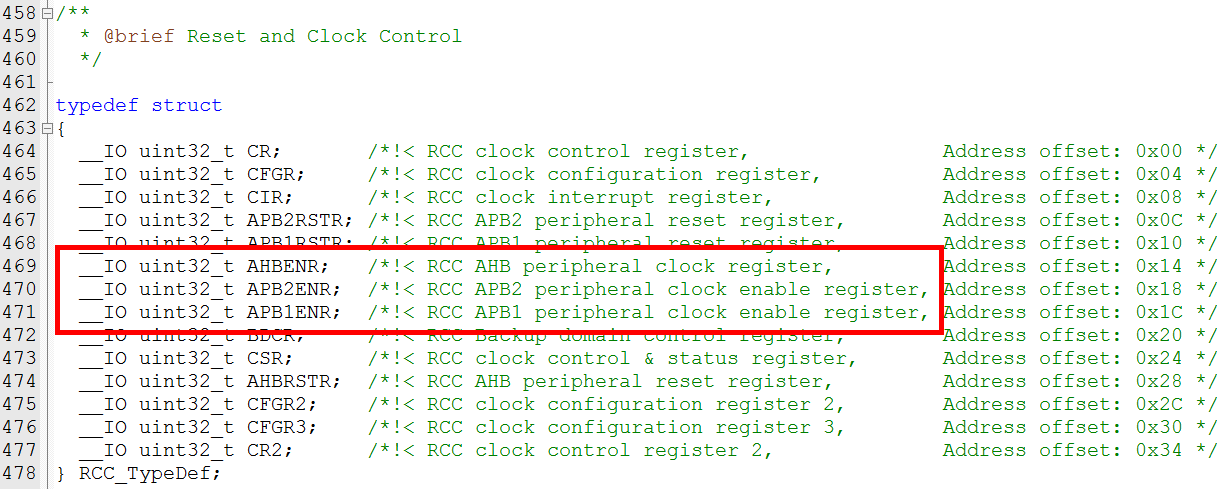
\includegraphics[width=\textwidth]{rccStruct}
    \caption{RCC structure with peripheral clock enable registers highlighted}
    \label{rccStruct}
\end{figure}

% PASSIVE, REVISE
These three registers control the clock signals to all other peripherals, except for those in the ARM-core itself. The peripherals they control are organized by what system communications bus they are connected to. Some high-speed peripherals such as memory control, are connected directly to the \textit{Advanced High-performance Bus} (AHB). However, most peripherals are connected to one of two \textit{Advanced Peripheral Busses} (APB).

% PASSIVE
On the STM32F0, the GPIO peripherals are located on the AHB bus. However, in other architectures and brands, they may be located on the APB.

\begin{example}[Enabling a Peripheral Clock in the RCC]
    The following enables the peripheral clock for the GPIOB peripheral. Notice that a defined bit name was used instead of a simple bitmask. In many cases using these definitions results in clearer code.

    \ilcode{RCC->APB1ENR |= RCC\_APB1ENR\_TIM2EN;    // Enable peripheral clock to TIMER2}
    \smallskip
    %\texttt{RCC->AHBENR |= RCC\_AHBENR\_GPIOAEN;    // Enable peripheral clock to GPIOC}
\end{example}

\subsection{Slowing the System Down}
Even though the STM32F072 operates at a far slower clock rate than a conventional computer, it executes instructions fast enough that a simple pin toggling loop will flash the LED's faster than the human eye can see. Because of this, we'll have to introduce our own methods of adding delay into the program..

\subsubsection{Delay Loops}
% PASSIVE, REVISE
One simple (and very inefficient) way of adding delay into a program is to make the processor do lots of useless work in a \textit{busy loop}. A typical method of implementing a busy loop is to repeatedly increment a number until a limit is reached.

Unfortunately, compilers are pretty good at detecting and removing ``useless'' code that doesn't seem to be used anywhere else in the program. To help force the compiler to leave a delay loop alone, you will need to tag the loop variable as \textit{volatile}. One of the uses of the volatile keyword is to tell the system that the tagged variable has desired side-effects that the compiler may not see. Without this keyword, the compiler will optimize and remove structures such as delay loops.

%\colorbox{gray!20!white}{
%    \centering
%    \begin{minipage}{\linewidth}
%        \lstinline@volatile int i;@ \\
%        \lstinline@for(i=0; i < 100000; i++)\{\}@ 
%    \end{minipage}
%}

\smallskip
\colorbox{gray!20!white}{
    \centering
    \parbox{\linewidth-2\fboxsep}{
        \lstinline@volatile int i;@ \\
        \lstinline@for(i=0; i < 100000; i++)\{\}@ 
    }
}
\smallskip

In practice, delay loops are one of the most least-effective ways to introduce delay into a program. If possible, avoid using delay loops if hardware timing capabilities are available. 

\begin{warning}
    Always use the HAL library delay functions when blocking delays are required. Do not use busy-loops when timing hardware is available.
\end{warning}

\subsubsection{Hardware SysTick Delay}

% PASSIVE
The \textit{SysTick} timer peripheral is a device which raises a system signal at a configurable periodic rate. Because the time duration between these signals is known, the SysTick is often used as an application heartbeat. The HAL library uses the SysTick to trigger periodic tasks such as updating a global system time variable. 

As seen in the ``blinky'' example, the infinite loop calls the \texttt{HAL\_Delay()} function. This function is one of the delay mechanisms in the HAL library and halts the execution of a program by the number of milliseconds given as an argument. 

\ilcode{HAL_Delay(200); // Delay 200ms}
%\smallskip

% PASSIVE
Although these labs will typically avoid using the HAL library resources, it is encouraged that user applications make use of the HAL delay functions. One of the exercises in the next lab on interrupts will explore writing a similar delay function using the SysTick peripheral. However, since the HAL delay system is automatically initialized during the clock speed configuration, it is easier to use the preexisting functionality for most purposes. 

\subsection{Standard Integer Types}

% REVISE
While most of the C-standard variable types work properly on embedded systems, there is always the possibility that they are not the size (number of bits) usually expected. For example, similar to many systems an ``int'' on the STM32F0 is 32-bits wide. However, on 8-bit processors, an integer type is typically 8 or 16 bits. To avoid confusion and very subtle bugs, most toolchains define explicit numeric types. Figure \ref{types} shows the integer types defined and used within ST's provided files.

\code{./files/types.h}{Integer variable types defined in ST Microelectronics support files.}{types}
%\code{./files/types.h}
\begin{warning}
    Avoid floating-point types when possible! Many embedded devices do not have hardware support for floating-point mathematics and must emulate it with large and slow code libraries. Higher-end devices such as the STM32F4 family of chips have a hardware floating-point unit. (FPU) 
\end{warning}

\subsection{``Debouncing'' External Signals} \label{bounce_section}

\begin{figure}[]
    \centering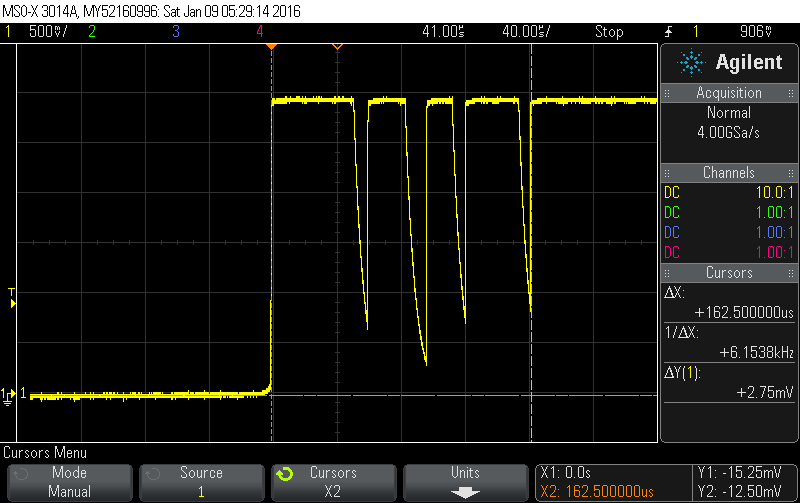
\includegraphics[width=\textwidth]{bounce}
    \caption{Signal bounce on button press.}
    \label{bounce}
\end{figure}

% PASSIVE, REVISE
One complication when working with physical devices such as buttons is often their transitions are not cleanly defined. Most mechanical buttons and switches ``bounce'' when they are pressed, unfortunately, most processors are fast enough to be able to see these bounces as multiple presses! Figure \ref{bounce} shows an oscilloscope trace captured from one of the Discovery board's buttons.

% PASSIVE
There are multiple ways of dealing with bouncing signals. The Discovery board has circuit footprints available for creating a hardware low-pass filter. However, these pads are not populated with components, and it is necessary to deal with the bouncing signal in software.

% REVISE
One simple way to debounce an input signal is to use a shifted bit-vector. A shifted bit vector is an unsigned integer variable which has its lowest bit (rightmost) set to the state of the input signal every iteration through the program loop. As time passes (or each loop iteration) the variable is shifted by one bit to the left. This results in the variable's value representing the input pin's state throughout the bouncing interval. We can reject the bouncing by triggering the code only on steady state values of the variable. (For example: 0xFFFF or 0x0000) Figure \ref{debounce} shows an example debounce routine using a shifted bit-vector.

\code{./files/debounce.c}{Debouncing method using shifted bit-vector}{debounce}

%\section{Hello World: Writing Basic I/O Code}
%\section{Section Activity: Writing Basic I/O Code}
\section{Lab Assignment: Writing Basic I/O Code}

These exercises explore two basic operations of the GPIO: Blinking LEDs and reading the state of a pushbutton.
After completing these tasks, make sure to show the lab assistant! Most of your points for this lab will come from demonstrating that your code works. 
\begin{warning}
As mentioned earlier, \textbf{you will need to write your applications using \textit{only} peripheral register access.} The single exception to this is the \texttt{\textbf{HAL\_Delay()}} function.
\end{warning}

There are multiple ways to approach these exercises. Many lab assignments begin as empty projects, however, it is recommended for this first application that you begin with the provided ``blinky'' example code and make incremental changes from the HAL library calls to bitwise operations on peripheral registers.

% REVISE
The benefit of converting a working example is that it becomes possible to compile and test the application after replacing each line of code. This breaks down the possible sources of error into manageable portions. 

\subsection{Configuring a GPIO Pin to Output and Blink an LED}

Your goal in this lab assignment is to recreate the blinking demo using the red and blue LEDs on the Discovery board. 

If beginning with the example ``blinky'' application, the assignment can be broken down into the following steps:

\subsubsection{Converting the HAL Library Calls to Register Access}
\begin{enumerate}
    
    \item Use the RCC to enable the GPIOC peripheral clock.
    \begin{itemize}
        \item Remove the \texttt{\_\_HAL\_RCC\_GPIOC\_CLK\_ENABLE()} HAL library macro.
        \item Use the stm32f072xb.h header file to determine the register that enables the GPIOC peripheral clock.
        \item Set the appropriate bit using bitwise operations and either a bitmask or defined bit name. 
    \end{itemize}
    \item Configure the LED pins to slow-speed, push-pull output mode without pull-up/down resistors.
    \begin{itemize}
        \item Remove the \texttt{GPIO\_InitTypeDef} struct and \texttt{HAL\_GPIO\_Init()} function call.
        \item The green and orange LEDs are on pins PC8 and PC9.
        \item Set the pins to general-purpose output mode in the MODER register. 
        \item Set the pins to push-pull output type in the OTYPER register.
        \item Set the pins to low speed in the OSPEEDR register. 
        \item Set to no pull-up/down resistors in the PUPDR register. 
    \end{itemize}

    Each register map in the peripheral reference manual documents the starting state of bits in the register. Although clearing bits that should already be zero is not always necessary, it is good style to ensure that every bit is in a known state.  
    \medskip

    \item Initialize one pin logic high and the other to low.
    \begin{itemize}
        \item Remove the \texttt{HAL\_GPIO\_WritePin()} function call.
        \item Use either the ODR or BSRR register.  
    \end{itemize}
    \item Toggle both pin output states within the endless loop.
    \begin{itemize}
        \item Remove the \texttt{HAL\_GPIO\_TogglePin()} function call.
        \item Use either the ODR or BSRR register. 
    \end{itemize}
    \item Leave the HAL delay function within the loop. Otherwise, the LEDs will toggle too rapidly to see. Feel free to change the duration to reasonable values.
\end{enumerate}


\subsubsection{Changing to the New LEDs}

\begin{enumerate}
    \item Use the \textit{Hardware Layout} section of the Discovery board manual to find the pins connecting to the red and blue LEDs.  
    \begin{itemize}
        \item Page 13 of the Discovery board manual lists the STM32F0 pins used for LEDs.
        \item The red LED is labeled as \textit{LD5} and the blue as \textit{LD6} on the Discovery board.
        \item All LED pins are in the GPIOC peripheral. 
    \end{itemize}
    \item Update the pin initialization and toggle code to use the new pins.
\end{enumerate}


\subsection{Configuring a GPIO Pin to Input and Reading a Button}

Your goal in this portion of the lab assignment is to change your version of the flashing LED program, such that the LEDs toggle on a button press instead of a set delay. This can be broken down into the following steps:

\begin{enumerate}
    \item Use the \textit{Hardware Layout} section of the Discovery board manual to find the pin connected to the ``USER'' button.
    \begin{itemize}
        \item The user button is labeled as \textit{B1} on the Discovery board.
        \item Search through and find the material on available buttons. 
    \end{itemize}
    \item Use the RCC to enable the clock to the appropriate GPIO peripheral.
    \item Configure the button pin to input mode with the internal pull-down resistor enabled.
    \begin{itemize}
        \item Set the pins to input mode in the MODER register. 
        \item Set the pins to low speed in the OSPEEDR register. 
        \item Enable the pull-down resistor in the PUPDR register. 
    \end{itemize}
    \item Monitor the button pin input state within the endless program loop.
    \begin{itemize}
        \item Use the IDR register.  
    \end{itemize}
    \item Toggle the LED pins when a button press is detected.
    \item Include a software debounce routine to prevent multiple toggles on a single button press.
    \begin{itemize}
        \item See section \ref{bounce_section} for an example debounce routine. 
    \end{itemize}
\end{enumerate}

% PASSIVE
After making these changes to the original application, there is no need for a long duration delay statement each loop iteration. However, some program delay is still required (few milliseconds) otherwise the button debouncing method shown in section \ref{bounce_section} will not operate properly. 

\begin{warning}
    Some GPIO peripherals contain pins with system critical functions. For example, GPIOA contains pins PA13 (SWDIO) \& PA14 (SWCLK) which are used by the debugging hardware to communicate with the STM32F0. 
    
    % PASSIVE
    When using GPIO peripherals with special functions, \textbf{do not modify the control bits for these pins!} This includes clearing the entire register to ensure that all unknown bit states are set to a known value. 
    
    If the configuration for PA13 and PA14 is modified, the debugger will no longer be able to program the Discovery board. If this occurs, it can be fixed using the standalone ST-Link utility.
\end{warning}

\end{document}
